\documentclass[review,authoryear,3p,times]{elsarticle}
% EJOR submission -- v3 draft (started 2026-08-14).
%
% v3 REFRAME. v2 (main.tex, retained UNMODIFIED -- it is untracked, do not
% overwrite) was built around two mechanisms: s-ccf (component-factored credit)
% and cfpk (forked simulator replay). v3 is built around ONE mechanism,
% cgae-cflow: run GAE along the token-provenance DAG instead of the trajectory
% index. It needs no forking, no hand-specified factorization, and ~1 ms/episode.
%
% WHAT CARRIES OVER FROM v2 NEAR-VERBATIM: Section 2 (related work, plus two new
% paragraphs), Section 3 (background, plus a GAE subsection), and Section 7 (the
% boundary-condition investigation, unchanged). Those are marked \portold.
%
% CLAIM DISCIPLINE (see ../EJOR_PAPER_OUTLINE_V3.md 6.0 and 6a-40): all ncopies
% and s1 numbers here are at the CONVERGED 40-epoch budget. The 15-epoch
% protocol produced a significant but spurious result and must not be reported
% as primary. In particular v2's "beats ccf" framing is RETIRED: at converged
% budgets cgae-cflow does not beat ccf, cgae, or cgae-cap.

\usepackage{amsmath,amssymb,amsthm}
\usepackage{graphicx}
\usepackage{booktabs}
\usepackage{algorithm}
\usepackage{algpseudocode}
\usepackage{xcolor}
\usepackage{tikz}
\usetikzlibrary{petri,positioning,arrows.meta,fit,backgrounds,calc}
\usepackage[hidelinks]{hyperref}

\newtheorem{proposition}{Proposition}
\newtheorem{corollary}{Corollary}
\newtheorem{assumption}{Assumption}
\newtheorem{remark}{Remark}
\newtheorem{lemma}{Lemma}
\newtheorem{definition}{Definition}

% --- estimator names -------------------------------------------------------
\newcommand{\cgae}{\textsc{cgae}}              % mean over successors
\newcommand{\cflow}{\textsc{cgae-cf}}          % THE METHOD: convex flow weights
\newcommand{\cflowraw}{\textsc{cgae-f}}        % predecessor-normalized (broken)
\newcommand{\cdag}{\textsc{cgae-dag}}          % exact closure semantics
\newcommand{\ccap}{\textsc{cgae-cap}}          % sub-stochastic ablation
\newcommand{\ccf}{\textsc{ccf}}
\newcommand{\sccf}{\textsc{s-ccf}}
\newcommand{\mcq}{\textsc{mc-q}}
\newcommand{\lrq}{\textsc{lrq}}
\newcommand{\cfgae}{\textsc{cfgae}}
\newcommand{\cfpk}{\textsc{cfpk}}

\newcommand{\Fscr}{\mathcal{F}}
\newcommand{\Ascr}{\mathcal{A}}
\newcommand{\Ex}{\mathbb{E}}
\newcommand{\Var}{\operatorname{Var}}
\newcommand{\Cov}{\operatorname{Cov}}
\newcommand{\desc}{\operatorname{desc}}
\newcommand{\anc}{\operatorname{anc}}
\newcommand{\pred}{\operatorname{pred}}
\newcommand{\suc}{\operatorname{succ}}
\newcommand{\own}{\operatorname{own}}

% --- drafting aids: make every gap LOUD -----------------------------------
% \gap{...}      a missing number or result, with what is needed
% \gapdisc{...}  a discussion paragraph that cannot be written until a gap fills
% \portold{}  content to be copied across from main.tex (v2)
\newcommand{\gap}[1]{{\color{red}\textbf{[GAP: #1]}}}
\newcommand{\gapdisc}[1]{%
  \par\medskip\noindent{\color{red}\textbf{[DISCUSSION PENDING]} #1}\par\medskip}
\newcommand{\portold}[1]{%
  \par\medskip\noindent{\color{blue}\textbf{[PORT FROM v2 main.tex: #1]}}\par\medskip}

\journal{European Journal of Operational Research}

\begin{document}

\begin{frontmatter}

\title{Causal-Order Advantage Estimation: Exploiting Token Lineage for
Credit Assignment in Reinforcement Learning for Dynamic Task Assignment}

\author[tue]{R. Lo Bianco}
\address[tue]{Eindhoven University of Technology, The Netherlands}

\begin{abstract}
Deep reinforcement learning is increasingly applied to dynamic task assignment:
routing stochastic streams of work to limited, contended resources. When such a
system is modelled as an Action-Evolution Petri Net, the simulator records, at no
extra cost, the \emph{provenance} of every token---which past decisions causally
influenced which rewards. Existing methods discard this and hand the net to
off-the-shelf policy-gradient learning as a black-box semi-Markov decision
process. Generalized Advantage Estimation then accumulates temporal-difference
errors along the \emph{trajectory index}, but in a system running many concurrent
cases the next decision usually belongs to a different case, so its error term is
largely noise with respect to the current action. We run the identical recursion
along the provenance DAG instead. The resulting estimator assigns each reward to
a single owner---making credit a return decomposition rather than a hindsight
Q-sample---and combines causal successors by a flow-weighted average normalized
over successors. We show that the natural formulation, which normalizes over
\emph{predecessors}, leaves the bootstrap coefficient unbounded and consequently
\emph{diverges} during training; bounding that coefficient is what is
necessary, and normalizing over successors is the canonical way to achieve it.
On five problem configurations spanning one to eight independent reward-bearing
components, causal-order estimation improves normalized return over
discount-matched PPO by $+0.19$ to $+0.51$ (paired, $20$ seeds, $p\le0.002$) on
the three most decomposable of them, and is statistically indistinguishable from
it on the two least, all while costing about one millisecond per episode. We
further show that a structural statistic computed before training---the number of
reward-bearing causal components---predicts where the method helps and where it
provably cannot, and we report a battery of falsified alternative explanations so
that the mechanism claim is auditable rather than asserted.
\end{abstract}

\begin{keyword}
reinforcement learning \sep credit assignment \sep dynamic task assignment \sep
Petri nets \sep decomposition \sep policy gradient
\end{keyword}

\end{frontmatter}

%===========================================================================
\section{Introduction}
%===========================================================================

Dynamic task assignment---deciding, repeatedly and under uncertainty, which
resource should serve which unit of work---is among the most widely studied
operational control problems in operational research, covering machine
scheduling, service operations, patient flow, order picking and vehicle
dispatching. Recent work models such problems as Action-Evolution Petri Nets
(A-E PNs) and solves them with deep reinforcement learning, which handles the
combinatorial, variable-dimension action spaces that classical policies struggle
with.

That line of work treats the learner as interchangeable. The net is compiled into
a semi-Markov decision process and handed to proximal policy optimization with
Generalized Advantage Estimation (GAE). In doing so it discards something the
formalism provides for free.

\paragraph{The credit-assignment problem in concurrent systems.}
GAE accumulates temporal-difference errors along the trajectory index,
$A_t = \delta_t + \gamma\lambda A_{t+1}$. In an A-E PN running many cases
concurrently, decision $t+1$ typically belongs to a \emph{different case} from
decision $t$: its reward, and hence its TD error, is driven by tokens the action
at $t$ never touched. Credit therefore propagates along wall-clock order while
causality flows along the provenance DAG. The consequence is variance that grows
with concurrency, and it is severe. At the converged training budget on our
scaling benchmark with four independent copies, discount-matched PPO reaches
normalized return $0.715 \pm 0.265$ and collapses on one seed in twenty, where
the estimator proposed here reaches $0.980 \pm 0.092$ and collapses on none. On
the most decomposable environment the same contrast is $0.161$ against $0.673$,
with PPO collapsing on $14$ seeds of $20$ and the proposed estimator on none.

\paragraph{What the formalism already records.}
An A-E PN simulation logs, for every token, which transition firing produced it
from which input tokens. This provenance DAG is not an addition to the model; it
is a by-product of executing it. It answers exactly the question credit
assignment asks: which earlier decisions could have influenced this reward?

\paragraph{Contributions.}
\begin{enumerate}
\item \textbf{Causal-order advantage estimation} (\cflow, Section~\ref{sec:method}):
GAE with the temporal successor replaced by the \emph{causal} successor, with
single-owner reward attribution and a convex flow-weighted combination over
successors. The credit factorization is \emph{derived} from provenance per
episode rather than hand-specified, requires no forked simulation, and costs
about one millisecond per episode---under $8\%$ of a training iteration, in which
the graph neural network dominates.

\item \textbf{Identification and repair of a normalization defect}
(Section~\ref{sec:theory}). The natural flow-weighted form normalizes weights
over the \emph{predecessors} of each node, which is what a token-conservation
argument yields. But the recursion sums over \emph{successors}, so the
coefficient multiplying the bootstrap is a row sum that the conservation
constraint does not bound. We show the resulting error is proportional to the
critic, so the estimator degrades as the critic improves, and we observe exactly
that: on the single-component environment the unnormalized form does not merely
underperform, it \emph{diverges}, with variance growing sixfold between training
budgets and one run falling from near-optimal to below random.

\item \textbf{An ablation ladder in which fidelity to the causal estimand is
nearly uncorrelated with learning performance} (Section~\ref{sec:exp}). The
variant that satisfies the target identity \emph{exactly} ranks second-worst of
nine and is beaten decisively, while the variant that satisfies it at $0.626$ is
statistically indistinguishable from six others---plain PPO among them. What
separates working from failing estimators is not faithfulness but whether the
error is bounded.

\item \textbf{A pre-training diagnostic.} The number of reward-bearing causal
components $K$, and the mean causal fan-out, are computable from a handful of
random rollouts. Together they predict both whether the method can help
($K>1$) and whether the choice of successor-combination rule matters at all
(fan-out $>1$). We report a case where fan-out is exactly $1$ and every variant
is provably bit-identical.

\item \textbf{A boundary characterization} (Section~\ref{sec:boundary}, carried
over): three independent routes to supplying the learner with more structure ---
potential-based reward shaping, structural input features, and a graph-actor
architectural fix --- each provably inert or empirically neutral on a
single-component bottleneck.
\end{enumerate}

\paragraph{Scope.} We deliberately do not claim superiority over prior
component-factored credit schemes. At converged training budgets \cflow{} is
statistically indistinguishable from \ccf{} and from the mean-combination
variant (Section~\ref{sec:exp}); the differences reported in earlier drafts of
this work were artifacts of a shorter training budget. What is established is
that causal-order estimation beats discount-matched PPO decisively where causal
structure exists, and that the successor normalization is necessary to avoid
divergence.

%===========================================================================
\section{Related work}
\label{sec:related}

\paragraph{DRL for dynamic task assignment and operational control.} A growing
literature applies DRL to scheduling, routing, and business-process
decision-making, typically encoding the problem instance as a graph consumed
by a graph neural network policy: greedy graph-embedding heuristics for
combinatorial construction \citep{khalil2017learning}, attention-based
routing policies \citep{nazari2018vrp}, and GNN-based dispatching for job-shop
scheduling \citep{zhang2020jobshop}, the last especially close in spirit to
our setting. \citet{mazyavkina2021survey} survey this broader RL-for-
combinatorial-optimization literature; \citet{bengio2021tour}, published in
this journal, give the methodological tour d'horizon our OR framing draws on
most directly. Within the A-E PN program, \citet{aepn2023} introduce the
formalism and a taxonomy of assignment archetypes, \citet{aepn_repr2025} give
a graph representation for infinite state/action spaces, and \citet{gympn2025}
provide a library supporting partial observability and multiple decisions.
Across this literature, the learning algorithm is almost universally a black
box on top of the graph encoding; the simulator's own execution trace---which
decisions caused which outcomes---is not itself treated as a source of
learning signal. Our contribution is orthogonal to and compatible with all of
the above: it is a credit-assignment mechanism, not a new policy architecture
or problem encoding.

\paragraph{Credit assignment in RL.} Return decomposition \citep{rudder2019}
learns to redistribute return along a trajectory via a return-predicting
model's contribution analysis; Hindsight Credit Assignment \citep{hca2019}
reweights past actions by their learned likelihood of having caused an
observed outcome. Both are \emph{learned} redistribution mechanisms trained
on correlational patterns across trajectories. Our mechanisms differ in
kind: token provenance in an A-E PN is not inferred, it is recorded exactly by
the simulator, so \cflow{}'s credit signal carries no approximation
error from the attribution step itself. This is close in motivation to
model-free counterfactual credit assignment \citep{ccadeep2021}, which
conditions value functions on future events to build low-variance
counterfactual baselines; Simulator-replay counterfactual credit (\cfpk{}, which we treat as related
rather than contributed work in this version) is the model-based analogue of the
same goal, made exact because the simulator is itself an available,
cheap-to-fork causal model. It sits at the exact end of the same spectrum, at a
simulation cost \cflow{} avoids entirely.

\paragraph{Factored / multi-agent credit.} Difference rewards
\citep{difference2002} credit each agent with its marginal contribution
relative to a counterfactual baseline; COMA \citep{coma2018} learns this
baseline via a centralized critic; value decomposition
\citep{vdn2018,qmix2018} factors a joint value across agents under additivity
or monotonicity constraints. These require the entity/agent partition to be
given. A more recent line does not: MACCA \citep{macca2024} casts the
generative process as a dynamic Bayesian network and \emph{learns} the causal
structure from offline data, using a structure predictor with sparsity
regularization to recover which state and action dimensions influence each
agent's reward.

The distinction we draw is therefore not \emph{given versus derived}---that
would misrepresent \citet{macca2024}---but \emph{learned versus recorded}.
MACCA estimates the causal structure statistically from
$\{s,o,a,R,s'\}$ tuples, so the recovered graph carries estimation error,
requires enough data to identify, and can be wrong. Token provenance in an
A-E PN is not estimated at all: the simulator writes down, for each firing,
exactly which tokens were consumed and produced, so the attribution step
contributes \emph{zero} approximation error and needs no data beyond the
episode being credited. The partition is also free to change shape per
episode as the realized case mix changes, and a single-agent problem (one
policy, many concurrent cases) is factored the same way a genuinely
multi-agent one would be.

\paragraph{Treating the simulator as more than a black box.} Two recent lines
share our premise---that a discrete-event simulator exposes structure worth
exploiting---while exploiting different structure.
\citet{diffdes2024} make the simulator \emph{differentiable} and compute
pathwise policy gradients through it for queueing-network control, reporting
gradient estimates orders of magnitude more accurate than REINFORCE-style
estimators and large sample-efficiency gains. That approach needs a
differentiable simulator and smooth surrogate event dynamics; ours needs only
that the simulator record token identity, which A-E PN execution already does,
and leaves the policy-gradient estimator otherwise untouched. The two are
complementary rather than competing: pathwise differentiation improves the
gradient of a given objective, whereas causal-order estimation changes which
rewards enter a decision's advantage in the first place.
\citet{eventdriven2026} address long-horizon control in semiconductor
fabrication with an event-driven temporal-difference formulation over an
interconnected process of discrete events, in a domain close to ours.

\gap{Position precisely against \citet{eventdriven2026} once its method
section has been read. The open question is whether its event-driven TD
formulation changes WHICH past decisions are credited for a reward (causal
attribution, i.e.\ our contribution) or only WHEN transition boundaries fall
(SMDP timing, which we also do and which is standard). If the former, the
novelty claim in Section~1 needs restating; if the latter, this paragraph
should say so explicitly. Do not submit without resolving this.}

\paragraph{Potential-based reward shaping.} \citet{ng1999shaping} prove that
adding a potential-based term to every step's reward cannot change an MDP's
optimal policy, for any potential function. We use the SMDP-discounted
generalization of this theorem not as a headline mechanism but as one of
three falsified alternative routes in our boundary-condition investigation
(Section~\ref{sec:boundary}): a theorem-safe, empirically counter-productive
result at practical training budgets, included because it isolates
sample-efficiency effects cleanly from the bias effects that are our main
concern in Section~\ref{sec:theory}.

\paragraph{Graph neural networks for combinatorial optimization and
heterogeneous actor-critic architectures.} GNNs are now a standard state
encoder for RL over combinatorial structures with variable size and topology
\citep{khalil2017learning,zhang2020jobshop}; our environments use a
heterogeneous variant, the Heterogeneous Graph Transformer
\citep{hu2020hgt}, encoding places and transitions as distinct node types.
Section~\ref{sec:boundary} documents an architectural finding of independent
interest: a per-node actor decoder combined with directed-only (non-reversed)
message-passing edges can be \emph{exactly} blind to state outside its
forward-reachable neighborhood, a limitation the critic (which pools) does
not share. To our knowledge this is not previously documented for
heterogeneous actor-critic graph architectures, and the argument is
orthogonal to the specific choice of GNN backbone.

\paragraph{Decomposition in operations research.} Dantzig--Wolfe decomposition
\citep{dantzig1960decomposition} and Benders decomposition
\citep{benders1962partitioning} break a hard, structured optimization problem
into a master problem and weakly-coupled subproblems along a hand-identified
block structure. \cflow{} applies the same idea to the policy-gradient
\emph{return}: decompose it along a block structure derived automatically,
per episode, from the simulator's own causal record, rather than a static
constraint matrix's block structure identified a priori.

% ======================================================================

\paragraph{Generalized advantage estimation, and deliberate bias.}
Our estimator is GAE with one substitution, so GAE is the closest technical
antecedent rather than background. Two features of it matter here. First, GAE
with $\lambda<1$ is \emph{itself} a biased estimator---$\lambda=1$ is the
unbiased Monte-Carlo case---and the biased settings are universally preferred in
practice. Second, the bias it introduces is a shrinkage by \emph{temporal}
distance, $\lambda^k$; the estimator below shrinks by \emph{causal} distance
instead. The precedent is therefore direct: we are not introducing bias into an
unbiased pipeline, we are relocating a shrinkage that is already there.

\paragraph{Biased estimators as the norm.}
It is worth stating plainly that deliberate bias is standard rather than
exceptional in this literature: the clipped surrogate objective of PPO, truncated
importance weights in off-policy actor-critic, reward clipping in value-based
control, restricted value factorizations in cooperative multi-agent learning, and
discounting below the true horizon as a form of regularization. In statistics the
same point is a theorem: shrinkage estimators dominate the unbiased maximum
likelihood estimator in mean-squared error. We rely on this framing in
Section~\ref{sec:theory}, where the estimator we ship is biased and the one that
is exactly unbiased performs worse.

\paragraph{Positioning against factored and counterfactual credit.}
Difference rewards, counterfactual multi-agent baselines and value-decomposition
networks all require the entity partition to be supplied. Our factorization is
\emph{read off} the provenance DAG per episode. Simulator-replay counterfactual
credit obtains exact per-decision differences by forking the simulator; it sits
at the exact end of the same spectrum, at a cost in simulation we avoid.

%===========================================================================
\section{Background}
\label{sec:background}

Because Action-Evolution Petri Nets are not yet widely known, we describe the
formalism intuitively before defining the learning problem.

\paragraph{Petri nets and colored tokens.} A Petri net is a bipartite directed
graph of \emph{places} (drawn as circles) and \emph{transitions} (drawn as bars),
connected by arcs. Places hold \emph{tokens}; in a \emph{colored} net each token
carries typed data---a task's type, a resource's identity. A transition is
\emph{enabled} when its input places jointly hold a matching combination of
tokens, called a \emph{binding}; \emph{firing} the transition consumes that
binding and produces new tokens in its output places. The distribution of tokens
over places---the \emph{marking}---is the system state, and it evolves as
transitions fire.

\paragraph{The action/evolution split.} An Action-Evolution Petri Net (A-E PN)
\citep{aepn2023} partitions the transitions into two kinds and adds a global
clock. \emph{Evolution} transitions model the exogenous dynamics: they fire
automatically according to stochastic, timed rules---task arrivals, service
completions---advancing the clock. \emph{Action} transitions model the
controllable decisions: whenever several action bindings are simultaneously
enabled, an external \emph{policy} selects which one to fire. Selected firings may
carry a scalar \emph{reward}. Figure~\ref{fig:aepn} shows a minimal assignment
net: a waiting task and a free resource are consumed by an \emph{assign} action
transition---the decision of which task to serve with which resource---producing
a \emph{busy} token; an evolution transition \emph{complete} later frees the
resource (returning it to the pool) and emits a reward.

\paragraph{The induced SMDP.} Executing an A-E PN therefore alternates between the
environment evolving the marking (evolution firings that advance the clock) and
the agent choosing among enabled action bindings---exactly a semi-Markov decision
process (SMDP). We write $s_d$ for the marking at decision $d$, $a_d$ for the
chosen binding, and $u_d$ for its clock; delayed rewards are discounted by the
SMDP factor $\rho_d(t)=e^{-\beta\max(0,\,t-u_d)}$. Dynamic task assignment
problems---matching stochastic task streams to contended resources---map onto
this template directly \citep{aepn2023,aepn_repr2025,gympn2025}. Because the
simulator is a deterministic function of the marking, the clock, and the
(recorded) exogenous random draws, it can be \emph{snapshotted and re-run}
from any decision point under an alternative action---the capability
\cfpk{}'s forking (Section~\ref{sec:method}) relies on, and a further
consequence of the same executable-model property that makes A-E PN a
unified modeling-and-solving framework in the first place.

\begin{figure}[t]
\centering
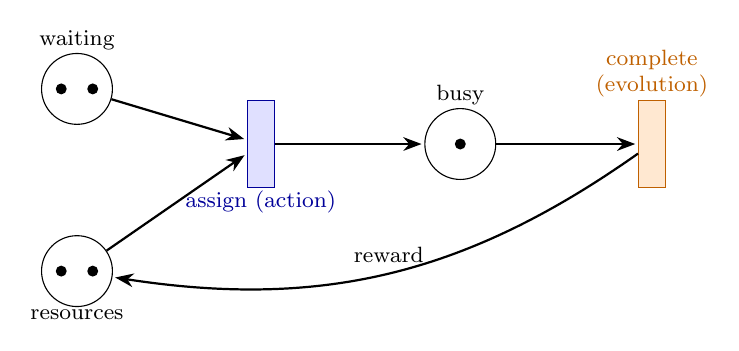
\begin{tikzpicture}[>=Stealth,node distance=1.5cm,
  place/.style={circle,draw,minimum size=9mm,inner sep=1pt},
  tok/.style={circle,fill=black,inner sep=1.4pt},
  act/.style={rectangle,draw=blue!60!black,fill=blue!12,minimum width=3.4mm,minimum height=11mm},
  evo/.style={rectangle,draw=orange!75!black,fill=orange!18,minimum width=3.4mm,minimum height=11mm},
  arc/.style={->,thick,shorten >=1pt},
  every label/.style={font=\footnotesize,inner sep=1pt,align=center}]
  \node[place,label=above:{\footnotesize waiting}] (w) {};
    \node[tok] at ([xshift=-2mm]w.center){}; \node[tok] at ([xshift=2mm]w.center){};
  \node[place,below=1.4cm of w,label=below:{\footnotesize resources}] (r) {};
    \node[tok] at ([xshift=-2mm]r.center){}; \node[tok] at ([xshift=2mm]r.center){};
  \node[act,right=1.7cm of w,yshift=-0.7cm,label=below:{\footnotesize\color{blue!60!black}assign (action)}] (a) {};
  \node[place,right=1.9cm of a,label=above:{\footnotesize busy}] (b) {};
    \node[tok] at (b.center){};
  % label placed ABOVE and split over two lines: below the node it collided with
  % the reward arc sweeping back to `resources`, and a single line was wide
  % enough to reach the `busy` label.
  % Colour set as a node option, not an inline \color: a \color declaration does
  % not survive the \\ line break inside a label node.
  \node[evo,right=1.8cm of b,yshift=0cm,
        label={[text=orange!75!black]above:{\footnotesize complete\\(evolution)}}] (c) {};
  \draw[arc] (w) -- (a);
  \draw[arc] (r) -- (a);
  \draw[arc] (a) -- (b);
  \draw[arc] (b) -- (c);
  \draw[arc] (c) to[bend left=22] node[above,font=\footnotesize] {reward} (r);
\end{tikzpicture}
\caption{A minimal A-E PN for task assignment. Circles are places holding colored
tokens; bars are transitions. The \emph{assign} \textbf{action} transition
(blue) is a decision point: the policy chooses which waiting task to bind to which
free resource. The \emph{complete} \textbf{evolution} transition (orange) fires
automatically after a stochastic delay, returns the resource, and emits a reward.}
\label{fig:aepn}
\end{figure}

\paragraph{Policy gradient over A-E PN.} The policy $\pi_\theta$ is a graph neural
network over the assignment-graph representation \citep{aepn_repr2025}, trained
by PPO \citep{ppo2017} with generalized advantage estimation \citep{gae2016}. The
canonical unbiased gradient estimator credits each decision with its
reward-to-go against a learned baseline $V(s_d)$; both mechanisms below modify
only how that reward-to-go is computed.

% ======================================================================

\paragraph{Provenance DAG.}
Executing an A-E PN produces a record, for each firing, of the input tokens
consumed, the output tokens produced, the firing time, and any reward emitted.
Writing $\Ascr$ for the set of \emph{agent decisions} in an episode, indexed in
firing order with clock values $u_d$, the token history induces a directed
acyclic graph on $\Ascr$: token identity links each consumed token back to the
firing that produced it, transitively through non-decision (forced and
evolution) firings.

\paragraph{Generalized advantage estimation.}
For completeness, GAE forms
$A_t = \sum_{k\ge 0}(\gamma\lambda)^k \delta_{t+k}$ with
$\delta_t = r_t + \gamma V(s_{t+1}) - V(s_t)$, computed by the backward
recursion $A_t = \delta_t + \gamma\lambda A_{t+1}$. The substitution in
Section~\ref{sec:method} replaces the successor $t+1$ in this recursion.

%===========================================================================
\section{Method: causal-order advantage estimation}
\label{sec:method}
%===========================================================================

% The lineage / causal-order mechanism figure. \input from main_v3.tex.
% Panel (a) is the paper's central idea in one picture: GAE bootstraps from the
% TEMPORAL successor, which in an interleaved system belongs to a different case;
% causal-order estimation bootstraps from the CAUSAL successor instead.
% Panel (b) is the normalization that Proposition 1 turns on.
\begin{figure}[t]
\centering
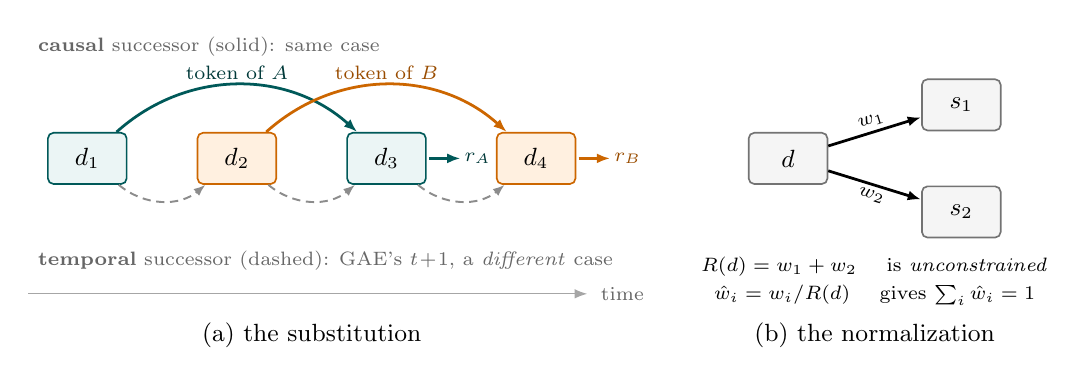
\begin{tikzpicture}[
  dec/.style={draw, rounded corners=2pt, minimum height=6.5mm,
              minimum width=10mm, align=center, font=\small, line width=0.6pt},
  caseA/.style={dec, fill=teal!8,   draw=teal!70!black},
  caseB/.style={dec, fill=orange!12, draw=orange!80!black},
  plain/.style={dec, fill=black!4,  draw=black!55},
  causalA/.style={-{Latex[length=1.7mm]}, line width=1.0pt, teal!70!black},
  causalB/.style={-{Latex[length=1.7mm]}, line width=1.0pt, orange!80!black},
  temporal/.style={-{Latex[length=1.5mm]}, densely dashed, line width=0.7pt,
                   black!45},
  tag/.style={font=\scriptsize, inner sep=1.5pt},
  note/.style={font=\scriptsize, black!60},
]

% ================= panel (a): temporal vs causal successor =================
\node[caseA] (d1) at (0,0)   {$d_1$};
\node[caseB] (d2) at (1.9,0) {$d_2$};
\node[caseA] (d3) at (3.8,0) {$d_3$};
\node[caseB] (d4) at (5.7,0) {$d_4$};

% causal recursion: solid arcs ABOVE, one per case
\draw[causalA] (d1) to[bend left=42]
  node[midway, above, tag, teal!45!black] {token of $A$} (d3);
\draw[causalB] (d2) to[bend left=42]
  node[midway, above, tag, orange!60!black] {token of $B$} (d4);

% temporal recursion: dashed arcs BELOW, consecutive, with visible heads
\foreach \a/\b in {d1/d2, d2/d3, d3/d4}
  \draw[temporal] (\a) to[bend right=40] (\b);

% rewards, emitted at the consuming decision
\draw[causalA] ($(d3.east)+(0.03,0)$) -- ++(0.40,0)
  node[right, tag, teal!45!black, inner sep=1pt] {$r_A$};
\draw[causalB] ($(d4.east)+(0.03,0)$) -- ++(0.40,0)
  node[right, tag, orange!60!black, inner sep=1pt] {$r_B$};

% legends for the two arrow families
\node[note, anchor=west, align=left] at (-0.75,1.42)
  {\textbf{causal} successor (solid): same case};
\node[note, anchor=west, align=left] at (-0.75,-1.30)
  {\textbf{temporal} successor (dashed): GAE's $t\!+\!1$, a \emph{different} case};

\draw[-{Latex[length=1.6mm]}, black!35] (-0.75,-1.72) -- (6.35,-1.72);
\node[note, anchor=west] at (6.4,-1.72) {time};

\node[font=\small] at (2.85,-2.25) {(a) the substitution};

% ================= panel (b): the successor normalization =================
\begin{scope}[xshift=8.9cm]
  \node[plain] (dd) at (0,0)      {$d$};
  \node[plain] (s1) at (2.2,0.68) {$s_1$};
  \node[plain] (s2) at (2.2,-0.68){$s_2$};

  \draw[-{Latex[length=1.7mm]}, line width=1.0pt] (dd) --
    node[midway, above, sloped, tag] {$w_1$} (s1);
  \draw[-{Latex[length=1.7mm]}, line width=1.0pt] (dd) --
    node[midway, below, sloped, tag] {$w_2$} (s2);

  % formulas: \textstyle keeps the sum limits inline, so nothing collides
  \node[anchor=north, align=center, font=\scriptsize, inner sep=2pt]
    at (1.1,-1.18)
    {$R(d)=w_1+w_2$ \quad is \emph{unconstrained}\\[2pt]
     $\hat w_i = w_i/R(d)$ \quad gives $\textstyle\sum_i \hat w_i = 1$};

  \node[font=\small] at (1.1,-2.25) {(b) the normalization};
\end{scope}

\end{tikzpicture}
\caption{The mechanism. \textbf{(a)} Four decisions in wall-clock order, drawn
from two interleaved cases $A$ and $B$. Generalized advantage estimation
bootstraps along the dashed \emph{temporal} chain, so the TD error it charges to
$d_1$ is the one produced at $d_2$---a decision about a different case, whose
reward $d_1$ did not influence. The token $d_1$ produced is instead consumed at
$d_3$, where the reward $r_A$ is emitted. Causal-order estimation follows the
solid provenance edges, so $d_1$ is credited with $r_A$ and never with $r_B$.
Reward ownership is a partition---each reward is assigned to the latest decision
on its own lineage---so no reward is counted twice. \textbf{(b)} Where a
decision's tokens feed several later decisions, the edge weights must be
normalized \emph{over successors}. Token conservation constrains the sum over
each node's predecessors, which leaves the row sum $R(d)$ free; because $R(d)$
multiplies the bootstrapped value (Proposition~\ref{prop:s}), leaving it
unbounded makes the recursion diverge in training.}
\label{fig:lineage}
\end{figure}


\subsection{Causal successors}

Figure~\ref{fig:lineage} shows the construction on a short episode: the
trajectory index along which GAE ordinarily accumulates, and the provenance DAG
that replaces it. For a decision $d\in\Ascr$, define $s\in\suc(d)$ when $s$
consumes a token descending from an output token of $d$ with no intervening
decision---the \emph{nearest producer} relation. Forced firings and evolution transitions are
transparent: the backward walk passes through them to the decision that actually
caused the flow. This is a purely structural construction requiring no
token-value semantics and no assumption about what the tokens represent.

\begin{remark}[A known specification wrinkle, disclosed]
Under token-flow postponement, a \textsc{postpone} decision re-emits the entire
marking, so it stops the nearest-producer walk despite not having caused the
flow. Making it transparent recovers real causal edges---measured at $97$ per
episode on our single-component environment, with none lost---and is arguably the
correct graph. It nonetheless \emph{degrades} learning sharply
(Section~\ref{sec:exp}). We report this as a measured boundary of the
specification rather than resolving it.
\end{remark}

\subsection{Single-owner reward attribution}

Each reward $r_j$ is assigned to the \emph{latest} decision on its lineage,
$\own(j)=\arg\max_{d\in\Ascr(j)} u_d$, where $\Ascr(j)$ is the set of decisions
in $j$'s ancestry. Ownership is therefore a \emph{partition}: every reward is
counted exactly once. This is what makes the estimator a return decomposition
rather than a hindsight $Q$-sample, in which each decision on a lineage receives
the reward's full mass.

\subsection{The recursion}

Let $w(d\!\to\!s)$ be the share of $s$'s consumed tokens descending from $d$, so
that token conservation gives
\begin{equation}
\sum_{d\in\pred(s)} w(d\!\to\!s) = 1 .
\label{eq:predsum}
\end{equation}
Define the row sum and the \emph{successor-normalized} weights
\begin{equation}
R(d) = \sum_{s\in\suc(d)} w(d\!\to\!s), \qquad
\hat{w}(d\!\to\!s) = \frac{w(d\!\to\!s)}{R(d)},\qquad
\sum_{s\in\suc(d)}\hat{w}(d\!\to\!s)=1 .
\label{eq:sucsum}
\end{equation}
With $\rho(\Delta t)=e^{-\beta\Delta t}$ the SMDP discount applied at
\emph{causal} depth, the estimator is
\begin{equation}
A[d] \;=\; \mathrm{owned}[d] - V[d]
\;+\; \sum_{s\in\suc(d)} \hat{w}(d\!\to\!s)\,\rho(u_s-u_d)\,
      \bigl( V[s] + \lambda A[s] \bigr),
\label{eq:cflow}
\end{equation}
evaluated by a single backward pass over $\Ascr$ in decreasing clock order and
emitted as $Q[d]=A[d]+V[d]$, so it is consumed exactly as every other credit
scheme: the policy uses $A_d = Q[d]-V(s_d)$ and the value head regresses on
$Q[d]$. Because $V$ is fitted to the emitted $Q$, the critic converges to the
same object the recursion bootstraps through and the fixed point is
self-consistent. Algorithm~\ref{alg:cflow} states the procedure.

\begin{algorithm}[t]
\caption{Causal-order advantage estimation (\cflow)}
\label{alg:cflow}
\begin{algorithmic}[1]
\State \textbf{input:} decisions $\Ascr$ with clocks $u_d$; token history;
       critic values $V[\cdot]$; $\lambda$, $\beta$
\State build $\suc(\cdot)$ and $w(\cdot\!\to\!\cdot)$ by nearest-producer walk
       \Comment{$O(|E|)$}
\State $\mathrm{owned}[d]\gets 0$ for all $d$
\ForAll{rewards $r_j$}
  \State $\mathrm{owned}[\own(j)] \mathrel{+}= r_j$
         \Comment{latest decision on $j$'s lineage}
\EndFor
\ForAll{$d\in\Ascr$ in decreasing $u_d$}
  \If{$\suc(d)=\emptyset$} \State $A[d]\gets \mathrm{owned}[d]-V[d]$
  \Else
    \State $R\gets\sum_{s\in\suc(d)} w(d\!\to\!s)$
    \State $A[d]\gets \mathrm{owned}[d]-V[d]
            +\sum_{s} \tfrac{w(d\to s)}{R}\rho(u_s\!-\!u_d)(V[s]+\lambda A[s])$
  \EndIf
\EndFor
\State \textbf{return} $Q[d]=A[d]+V[d]$
\end{algorithmic}
\end{algorithm}

\subsection{Properties}

\begin{itemize}
\item \textbf{Chain-exact.} Where every causal edge has out-degree one and unit
weight, $\hat w\equiv 1$ and \eqref{eq:cflow} is ordinary SMDP-GAE. Verified to
floating point on real traces.
\item \textbf{The mean variant is a special case.} Under equal inflow shares
$\hat w = 1/|\suc(d)|$, which is the mean-over-successors combination
(\cgae). The mean is therefore not an underived rival but the equal-share
instance of \eqref{eq:cflow}.
\item \textbf{Cost.} Approximately one millisecond per episode; under $8\%$ of a
training iteration.
\item \textbf{Postponement} receives the SMDP temporal-difference advantage
$e^{-\beta\tau}V(s')-V(s)$ rather than a lineage credit, for consistent support.
\end{itemize}

%===========================================================================
\section{Theoretical analysis}
\label{sec:theory}
%===========================================================================

\subsection{A common form for the estimator family}

Every variant we consider is a choice of edge coefficient $c(d\!\to\!s)$ in
\eqref{eq:cflow}. Unrolling with $\lambda=1$ and $V\equiv 0$,
\begin{equation}
Q[d] \;=\; \sum_{j\,:\,\own(j)\in\desc^{*}(d)} c_d(j)\,\rho(u_j-u_d)\,r_j,
\qquad
c_d(j)=\!\!\sum_{\text{paths } d\rightsquigarrow \own(j)}\ \prod c ,
\label{eq:unroll}
\end{equation}
so a variant is characterized by the total path weight it places on each
descendant's owned reward. Table~\ref{tab:family} lists the family.

\begin{table}[t]
\centering
\caption{The estimator family, and the two sums that matter.}
\label{tab:family}
\begin{tabular}{llcc}
\toprule
variant & $c(d\!\to\!s)$ & $\sum_{\pred(s)} c$ & $\sum_{\suc(d)} c$ \\
\midrule
\cdag  & $1$ (closure, set semantics)      & ---            & convex \\
\cflow & $w/R$                             & unbounded      & $=1$ exactly \\
\cgae  & $1/|\suc(d)|$                     & unbounded      & $=1$ exactly \\
\ccap  & $w/\max(R,1)$                     & $\le 1$        & $\le 1$ \\
\cflowraw & $w$                            & $=1$ exactly   & \textbf{unbounded} \\
\bottomrule
\end{tabular}
\end{table}

\subsection{The causal partition, the estimand, and its unbiasedness}
\label{sec:estimand}

Everything below is stated relative to one reference estimator, which we define
here and prove unbiased. Section~\ref{sec:relative} then measures how far the
shipped estimator departs from it.

\paragraph{Descendants and causal components.}
Write $\desc(d)$ for the set of decisions reachable from $d$ under the
successor relation of Section~\ref{sec:method}, and
$\desc^{*}(d)=\desc(d)\cup\{d\}$ for its reflexive closure. Separately, build an
\emph{undirected} graph on $\Ascr$ with an edge $(d,d')$ whenever some reward
$r_j$ has both $d$ and $d'$ on its lineage, i.e.\ $\{d,d'\}\subseteq\Ascr(j)$.
Its connected components partition the decisions into \emph{causal components}
$C_1,\dots,C_M$; write $c(d)$ for the component of $d$. Because the whole
ancestry of a reward is joined into one component, every reward with
$\Ascr(j)\neq\emptyset$ has a well-defined component $c(j):=c(d)$ for any
$d\in\Ascr(j)$; rewards with empty ancestry are policy-independent constants and
drop out of the gradient. Note $\desc^{*}(d)\subseteq c(d)$---a causal
descendant shares a lineage with $d$, hence a component---so scoping credit to
the descendant closure discards at least as much as scoping it to the
component, and strictly more whenever a component holds two decisions neither
of which descends from the other.

\begin{definition}[The structural statistic $K$]
\label{def:k}
$K$ is the number of causal components containing at least one reward, computed
per episode and averaged over rollouts of an untrained policy. It is therefore
a real number rather than an integer: on the $N$-copies benchmark $K=N$ holds
per episode when every copy happens to emit a reward, and the reported means
$2.0$, $3.3$ and $6.3$ for $N=2,4,8$ sit at or below $N$ for that reason. No
training and no reward model beyond the simulator's own log is required to
compute it.
\end{definition}

\paragraph{The two reward-to-go signals.}
For decision $d$ let
\[
  G_d^{\mathrm{full}}=\sum_{j:\,t_j\ge u_d}\rho_d(t_j)\,r_j,
  \qquad
  \Delta_d=\sum_{\substack{j:\,t_j\ge u_d\\ c(j)\neq c(d)}}\rho_d(t_j)\,r_j ,
\]
so that $G_d^{\mathrm{full}}$ is the ordinary SMDP return-to-go---the signal PPO
and the lineage ablation \mcq{} use---and $\Delta_d$ is the part of it generated
by components other than $d$'s. Write $\Fscr_d$ for the history up to but
excluding $a_d$, so that $s_d$ is $\Fscr_d$-measurable and $a_d$ is drawn given
$\Fscr_d$. We take as given the policy-gradient theorem in its causality
(GPOMDP) form, that $\sum_d \nabla\log\pi(a_d\mid s_d)(G_d^{\mathrm{full}}-V(s_d))$
is unbiased for $\nabla_\theta J$; every claim below is relative to it.

\begin{assumption}[Component mean-exogeneity]
\label{as:exo}
For every decision $d$,
$\;\Ex[\Delta_d \mid \Fscr_d,\,a_d] = \Ex[\Delta_d \mid \Fscr_d]$: given the
pre-action history, the \emph{expected} cross-component future reward does not
depend on which action is taken at $d$.
\end{assumption}

This is the assumption referred to throughout as (A1), and A-E PN semantics
argue for it rather than merely permitting it. A reward $r_j$ is a deterministic
function of the tokens consumed at its firing, and each of those tokens' entire
histories is recorded in the provenance DAG; hence $r_j$ can be causally
influenced by $a_d$ only if some descendant of $a_d$ lies on $j$'s lineage---only
if $d\in\Ascr(j)$, which by construction of the partition means $c(j)=c(d)$. A
cross-component reward therefore has no causal path from $a_d$, and neither its
value nor its component membership can be altered by $a_d$ (a lineage link to $d$
would have placed it in $c(d)$ in the first place). The one residual channel is
the exogenous randomness driving cross-component events---arrival types, service
durations---and Assumption~\ref{as:exo} asserts that those draws are, in
conditional mean, unaffected by $a_d$. Under the standard simulation model of
independent per-firing draws this holds; it is a statement about the
noise model, not about problem-specific structure. It can fail if a shared,
finite resource pool couples nominally separate streams, which is precisely the
$K=1$ regime our negative control occupies.

\paragraph{The closure estimand.}
The first row of Table~\ref{tab:family} is the $c\equiv1$ member of the family:
the $\lambda=1$, $V\equiv0$ estimator that credits $d$ with each descendant's
owned reward exactly once, with no path weighting at all,
\begin{equation}
  A^{\star}[d] \;=\; \sum_{j\,:\,\own(j)\in\desc^{*}(d)} \rho_d(t_j)\,r_j .
  \label{eq:star}
\end{equation}
It is realized exactly by \cdag, whose measured identity ratio against
\eqref{eq:star} is $1.000$. Because ownership is a partition
(Section~\ref{sec:method}), each reward enters \eqref{eq:star} at most once
even when its owner is reachable from $d$ along several distinct paths---the
set semantics is what distinguishes it from the path-summing variants, and it
is why a re-convergent diamond's reward is counted once rather than twice.

\begin{proposition}[The closure estimand is unbiased]
\label{prop:star}
Under Assumption~\ref{as:exo}, the estimator
$\hat g^{\star}=\sum_{d}\nabla_\theta\log\pi_\theta(a_d\mid s_d)\bigl(A^{\star}[d]-V(s_d)\bigr)$
satisfies $\Ex[\hat g^{\star}]=\nabla_\theta J(\theta)$ for any
$\Fscr_d$-measurable baseline $V$.
\end{proposition}

\begin{proof}
Write the discarded mass as
$G_d^{\mathrm{full}}-A^{\star}[d]=\Delta_d+\Xi_d$, where $\Delta_d$ collects the
cross-component rewards and
$\Xi_d=\sum \rho_d(t_j)r_j$ runs over the rewards $j$ with $t_j\ge u_d$,
$c(j)=c(d)$ and $\own(j)\notin\desc^{*}(d)$: those in $d$'s own component that
the closure nonetheless omits. It suffices to show each vanishes in the
gradient.

Fix $d$ and condition on $\Fscr_d$. Since $a_d$ is drawn given $\Fscr_d$ and
both quantities are realized afterwards,
\[
  \Ex\bigl[\nabla\log\pi_\theta(a_d\mid s_d)\,X_d \mid \Fscr_d\bigr]
  = \Ex_{a_d}\bigl[\nabla\log\pi_\theta(a_d\mid s_d)\,
    \Ex[X_d\mid\Fscr_d,a_d]\bigr]
\]
for $X_d\in\{\Delta_d,\Xi_d\}$. For $X_d=\Delta_d$ the inner expectation is
free of $a_d$ by Assumption~\ref{as:exo}. For $X_d=\Xi_d$, a reward $j$ in that
sum has $\own(j)\notin\desc^{*}(d)$; since $\own(j)$ is the \emph{latest}
decision on $j$'s lineage and the successor relation is time-forward, no
decision of $\Ascr(j)$ can lie in $\desc^{*}(d)$ at all, so no descendant of
$a_d$ is on $j$'s lineage. By the same A-E PN argument that justifies
Assumption~\ref{as:exo}---$r_j$ is a deterministic function of the tokens
consumed at its firing, whose histories are recorded---$r_j$ is then causally
uninfluenced by $a_d$, and its conditional mean is likewise free of $a_d$.

In both cases the inner expectation is some $\bar X_d$ not depending on $a_d$,
so the outer expectation is
$\bar X_d\,\Ex_{a_d}[\nabla\log\pi_\theta(a_d\mid s_d)\mid\Fscr_d]
 =\bar X_d\,\nabla_\theta\sum_a \pi_\theta(a\mid s_d)=\bar X_d\,\nabla_\theta 1=0$
by the score-function identity. The baseline term contributes zero by the same
identity. Summing over $d$ and taking total expectation gives the claim.
\end{proof}

\begin{remark}[What Proposition~\ref{prop:star} does and does not license]
It licenses \eqref{eq:star} as a reference point, and with it every
\emph{relative} statement in Sections~\ref{sec:bias} and \ref{sec:relative}. It
says nothing about the estimator we ship, which is biased relative to
\eqref{eq:star} by a quantity Proposition~\ref{prop:bias} bounds; and it says
nothing about performance---\cdag{} computes \eqref{eq:star} exactly and is the
second-worst arm we measured (Section~\ref{sec:exp}). Unbiasedness here is a
property of the estimand, not a recommendation.
\end{remark}

\subsection{Why the bootstrap coefficient must be bounded}

\begin{proposition}[Successor normalization]
\label{prop:s}
For the recursion \eqref{eq:cflow} with coefficient $c$, the coefficient
multiplying the bootstrap term at $d$ is $\sum_{s\in\suc(d)}c(d\!\to\!s)$. The
predecessor constraint \eqref{eq:predsum} does not bound this quantity. Writing
$\hat{G}(d)=\sum_s \hat w\,\rho\,(V[s]+\lambda A[s])$ for the estimator's own
bootstrapped continuation value, the unnormalized and normalized forms differ by
\begin{equation}
A_{\cflowraw}[d]-A_{\cflow}[d] \;=\; \bigl(R(d)-1\bigr)\,\hat{G}(d).
\label{eq:defect}
\end{equation}
\end{proposition}

\noindent The proof is immediate from $w = R\hat w$. Three consequences drive
everything in Section~\ref{sec:exp}.

\emph{(i) The error scales with the critic, not the reward.}
$\hat{G}(d)=O(V)=O(H\bar r)$ for remaining causal horizon $H$ and mean
per-decision reward $\bar r$, whereas the action-attributable signal is
$\mathrm{owned}[d]=O(\bar r)$. Hence
$|\text{error}|/|\text{signal}| \approx |R(d)-1|\cdot O(H)$. Because the error
grows with $V$, the estimator degrades \emph{as the critic improves}---a
divergence rather than a bias.

\emph{(ii) It does not cancel as a baseline.} $R(d)$ depends on the realized DAG
downstream of $d$, hence on the action at $d$. Forking every action at a decision
state under common random numbers, $R$ is identical across actions at only
$18.8\%$ (four independent copies) and $6.2\%$ (single component) of fork points.
An action-dependent term does not factor out through the score-function identity.

\emph{(iii) Successor normalization removes it identically.}
$\sum_s\hat w=1$ by construction, so $R\equiv 1$ and \eqref{eq:defect} vanishes
exactly---not in expectation. The mean variant is likewise protected.

\begin{remark}[The predecessor sum is a choice of estimand, not a defect]
\label{rem:p}
It is tempting to read \eqref{eq:predsum} as a second conservation requirement
and conclude that only $c=w/\max(R,1)$ is admissible. That is wrong.
$\sum_{\pred(s)}c>1$ means each of $s$'s joint causes is credited with the whole
continuation; since $s$ consumes a token from every predecessor, each is
\emph{necessary}, and crediting each in full is precisely the but-for
counterfactual that difference-reward methods use. Nothing in the
policy-gradient argument constrains advantages across \emph{different} decisions
to sum to anything. Empirically the distinction barely moves total credit mass:
$\sum_d Q[d]/G$ is $4.74$ for \cflowraw{} and $4.86$ for \cflow{} on the
single-component environment. Forcing the predecessor sum down (\ccap) costs
performance, as Section~\ref{sec:exp} shows.
\end{remark}

\subsection{Variance reduction, and the role of $K$}

The estimand of \eqref{eq:star} discards $\Delta_d$ without moving the expected
gradient. What it buys is variance, and the size of the purchase is governed by
$K$. The following isolates that mechanism in the simplest model that exhibits
it; it is an idealization, not a description of any particular environment.

\begin{proposition}[Component-scoped variance]
\label{prop:k}
Fix a decision $d$ and suppose the future reward-to-go splits as
$G_d^{\mathrm{full}}=\sum_{k=1}^{K}R_k$ with $d$ in component $1$, where $R_k$ is
component $k$'s discounted reward-to-go and, conditionally on $s_d$, the $R_k$
are mutually independent with variances $\sigma_k^2$. Let the baseline be any
$s_d$-measurable $V(s_d)$. Then
\[
  \Var\bigl(G_d^{\mathrm{full}}-V(s_d)\mid s_d\bigr)=\sum_{k=1}^{K}\sigma_k^2,
  \qquad
  \Var\bigl(R_1-V(s_d)\mid s_d\bigr)=\sigma_1^2 .
\]
If the components have comparable variance $\sigma_k^2\approx\sigma^2$,
component-scoped credit reduces the per-decision advantage variance by a factor
$\approx K$ and the gradient-noise standard deviation by $\approx\sqrt{K}$.
\end{proposition}

\begin{proof}
Conditionally on $s_d$ the baseline is a constant, so it does not affect either
variance. By conditional independence
$\Var(\sum_k R_k\mid s_d)=\sum_k \Var(R_k\mid s_d)=\sum_k\sigma_k^2$, which is
the first equality; the second is immediate. Under
$\sigma_k^2\approx\sigma^2$ the ratio is $K\sigma^2/\sigma^2=K$, and standard
deviation scales as the square root.
\end{proof}

\begin{remark}[The gap between the model and the estimator]
Two idealizations separate Proposition~\ref{prop:k} from what \cflow{} actually
computes. Conditional independence across components is stronger than
Assumption~\ref{as:exo}, which constrains only conditional means: (A1) is what
buys unbiasedness, independence is what buys the variance factor, and an
environment can satisfy the first while only approximately satisfying the
second. And \cflow{} scopes to $\desc^{*}(d)$, which is contained in $c(d)$ and
usually strictly smaller, so it discards more than the model does---which is why
the empirical gain is not a clean function of $K$ (Section~\ref{sec:scaling}).
The proposition should be read as identifying the mechanism and its governing
quantity, not as predicting an effect size.
\end{remark}

The scoping is directly observable. With
$S(d)=|\desc(d)|/|\{\text{decisions after }d\}|$, balanced components give
$S\approx 1/K$, and on the scaling benchmark with $N$ copies (where the copies are
independent by construction, so $K\le N$, with equality whenever every copy
emits a reward; see Definition~\ref{def:k}) $S$ measures $1.000, 0.472, 0.221, 0.114$ for $N=1,2,4,8$ against
$1/N = 1.000, 0.500, 0.250, 0.125$. At $N=1$, $S=1.000$ exactly: the estimator
provably performs no scoping, and indeed every method ties there.

\begin{remark}[$S$ is not $K$]
The single-component environment has $S=0.474$, essentially equal to the
two-copy benchmark's $0.472$, yet gains nothing while the latter gains. Scoping
away half the timeline buys variance reduction only if what is removed is
\emph{independent} of what is kept. $S$ measures how much is excluded; $K$
measures how much of it was independent.
\end{remark}

\subsection{Causal credit reduces total credit mass}

A natural objection to \eqref{eq:unroll} is that crediting every causal ancestor
must inflate credit relative to the return $G=\sum_j r_j$. It does, but far less
than the baseline it is compared against: under plain return-to-go a reward at
decision $k$ enters the advantage of all $k$ preceding decisions, giving
$\sum_t G_t \approx (n/2)G$ for $n$ decisions. Measured, $\sum_d Q[d]/G$ is
$39.78$, $21.23$ and $18.40$ for return-to-go on our three main environments
(against $n/2$ of $34.5$, $18$ and $14.5$) versus $4.34$, $4.32$ and $4.86$ for
\cflow---a four- to ninefold \emph{reduction}, tracking $1/S$ closely. The
residual is the variance-reduction mechanism viewed from the other side. Absolute
scale is in any case removed by per-batch advantage standardization.

\subsection{A bias bound for \cflow}
\label{sec:bias}

Proposition~\ref{prop:s} says the unnormalized form is unusable. It does not say
the normalized form is correct. This subsection bounds how far \cflow{} departs
from the closure estimand $A^\star$ of \eqref{eq:unroll}, i.e.\ from the variant
whose unbiasedness under Assumption~\ref{as:exo} is
Proposition~\ref{prop:star}. The bound is therefore \emph{relative}: it says how
much bias is added on top of that estimator, not that the result is unbiased.

\begin{assumption}[Time-forward causal edges]
\label{as:time}
$u_s > u_d$ for every causal edge $d\!\to\!s$.
\end{assumption}

\begin{assumption}[Bounded score]
\label{as:score}
$\lVert\nabla\log\pi(a\mid s)\rVert \le B$ for all $(s,a)$ visited.
\end{assumption}

Assumption~\ref{as:time} makes the DAG acyclic and, because
$\rho_{ds}=e^{-\beta(u_s-u_d)}$, makes the discount telescope along any path:
$\rho_{d s_1}\rho_{s_1 s_2}\cdots\rho_{s_{k-1}e} = \rho_{de}$, independently of
which path is taken. It is worth stating explicitly because the implementation
clamps negative time differences to zero, which would silently break telescoping
were an edge ever to point backwards in time.

\begin{lemma}[Path weights are visit probabilities]
\label{lem:visit}
Under Assumption~\ref{as:time}, $\hat W = [\hat w(d\!\to\!s)]$ is row-stochastic
on non-sink nodes and induces a Markov chain on $\Ascr$ with sinks absorbing.
For this chain,
\[
  c_d(e) \;=\; \Pr\bigl[\text{the walk started at } d \text{ visits } e\bigr]
  \;\in\;[0,1].
\]
\end{lemma}

\begin{proof}
Row-stochasticity is \eqref{eq:sucsum}. By Assumption~\ref{as:time} the DAG is
acyclic, so a walk visits any node at most once; consequently the events
$\{\text{the walk's initial segment is }\pi\}$, indexed by the distinct paths
$\pi: d\rightsquigarrow e$, are pairwise disjoint and their union is exactly the
event that the walk visits $e$. Each has probability
$\prod_{(x\to y)\in\pi}\hat w(x\!\to\!y)$, and summing gives $c_d(e)$. A
probability lies in $[0,1]$.
\end{proof}

Define the \emph{re-convergence deficiency} at $d$, in worst-case and
reward-weighted form,
\[
  \delta_d \;=\; \max_{e\in\desc(d)}\bigl(1-c_d(e)\bigr),
  \qquad
  \bar\delta_d \;=\;
  \frac{\sum_{e\in\desc^{*}(d)}\bigl(1-c_d(e)\bigr)\,\lvert\mathrm{owned}[e]\rvert}
       {\sum_{e\in\desc^{*}(d)}\lvert\mathrm{owned}[e]\rvert},
\]
and $\delta=\max_d \delta_d$. Both are computable from a handful of rollouts
without training.

\begin{proposition}[Bounded bias]
\label{prop:bias}
Under Assumptions~\ref{as:time} and \ref{as:score}, with $\lambda=1$ and
$V\equiv0$:
\begin{enumerate}
\item[(i)] $c_d(e)\in[0,1]$ for every $d$ and every $e\in\desc(d)$;
\item[(ii)] $\bigl\lvert A[d]-A^\star[d]\bigr\rvert
      \;\le\; \bar\delta_d \sum_{e\in\desc^{*}(d)}\lvert\mathrm{owned}[e]\rvert
      \;\le\; \delta_d \sum_{e\in\desc^{*}(d)}\lvert\mathrm{owned}[e]\rvert$;
\item[(iii)] the policy-gradient bias relative to the $A^\star$ estimator obeys
      \[
        \bigl\lVert \nabla J_{\cflow} - \nabla J_{\star}\bigr\rVert
        \;\le\; B\,\delta \sum_{e}\lvert\mathrm{owned}[e]\rvert\cdot
                \lvert\anc^{*}(e)\rvert
        \;\le\; B\,\delta\,n\,G_{\mathrm{abs}},
      \]
      with $G_{\mathrm{abs}}=\sum_j\lvert r_j\rvert$;
\item[(iv)] if every node of $\desc^{*}(d)$ has out-degree at most one, then
      $\delta_d=0$ and $A[d]=A^\star[d]$ \emph{exactly}. More generally
      $\delta_d=0$ if and only if $\desc^{*}(d)$ is totally ordered by
      reachability.
\end{enumerate}
\end{proposition}

\begin{proof}
(i) is Lemma~\ref{lem:visit}. For (ii), telescoping of $\rho$ gives
$A^\star[d]-A[d]=\sum_{e}\bigl(1-c_d(e)\bigr)\rho_{de}\,\mathrm{owned}[e]$;
take absolute values, use $\rho\le1$ and $0\le 1-c_d(e)\le\delta_d$, and note
the middle expression is exactly $\bar\delta_d$ times the total owned mass.
For (iii), the two estimators differ only through the summand, so
$\nabla J_{\cflow}-\nabla J_{\star}
 =\Ex\bigl[\sum_d (A[d]-A^\star[d])\nabla\log\pi_d\bigr]$; apply the triangle
inequality, then (ii) and Assumption~\ref{as:score}, and reindex the double sum
by owner, each $e$ being counted once per ancestor. For (iv), if out-degree is
at most one throughout $\desc^{*}(d)$ the walk is deterministic and visits every
descendant, so $c_d(e)=1$; conversely $c_d(e)=1$ for all $e$ says every maximal
walk from $d$ meets every descendant, which is total order by reachability.
\end{proof}

\paragraph{The bound is instrumented, and its equality case is observed.}
Table~\ref{tab:envs} reports mean $c_d(e)$ per environment. On multi-site
routing every decision has out-degree exactly one, and $c_d(e)=1.0000$ with
$\delta=0$: \cflow{} \emph{coincides with the unbiased closure estimand there},
so the headline realistic result is produced by an unbiased estimator. Where
out-degree exceeds one the deficiency appears and grows with fan-out: mean
$1-\bar c$ of $0.050$ at four copies and $0.285$ on the single-component
environment. We verified Lemma~\ref{lem:visit} numerically by simulating the
induced walk: Monte-Carlo visit frequencies match the closed form to
$\pm0.016$ at $4000$ samples, and $c_d(e)$ never left $[0,1]$.

\begin{remark}[What this does \emph{not} say]
\label{rem:notperf}
Proposition~\ref{prop:bias} bounds bias, not error, and certainly not
performance. \cdag{} attains $\delta=0$ by construction---it computes $A^\star$
exactly---and ranks second-worst of the nine arms in
Table~\ref{tab:ablation}. The proposition explains why \cflow{} is \emph{safe},
in the precise sense that its departure from the unbiased estimand is bounded by
a measurable structural quantity that vanishes on non-branching provenance
graphs. It does not explain why it is \emph{good}. Section~\ref{sec:exp} shows
the two questions have different answers.
\end{remark}

\subsection{What is still not proved}

The bound above is stated for $\lambda=1$ and $V\equiv0$. With a critic and
$\lambda<1$ the recursion becomes, by the same telescoping argument,
\[
  A[d] \;=\; \Ex_{\text{walk}}\Bigl[\textstyle\sum_{k\ge0}
             \lambda^{k}\rho_{d,X_k}\,\delta_{X_k}\Bigr],
  \qquad
  \delta_x=\mathrm{owned}[x]-V[x]+\Ex_{s}\bigl[\rho_{xs}V[s]\bigr],
\]
i.e.\ exactly GAE in expectation over the causal walk. The additional bias is
then the ordinary GAE bootstrap bias from an imperfect critic, which is neither
specific to this estimator nor bounded here.

\subsection{A dimensionless relative bound}
\label{sec:relative}

Proposition~\ref{prop:bias}(iii) bounds an absolute quantity, and its bound
scales with $n$ because the gradient is a sum of $n$ terms. That makes it weak.
One cannot simply divide by $\lVert\nabla J_{\star}\rVert$: near a stationary
point the denominator vanishes while the numerator need not, so no bound on the
\emph{ratio} of gradient norms can exist. The useful relative statement is about
\emph{direction}, and for this estimator it is available in closed form.

\begin{assumption}[Nonnegative owned rewards]
\label{as:pos}
$\mathrm{owned}[e]\ge0$ for all $e$.
\end{assumption}

This holds in every environment we study---throughput and completion rewards
are nonnegative, and we verified that no decision receives negative owned
reward in any measured episode---but it is a property of the reward model, not a
theorem, and estimators for cost-minimization problems with mixed-sign rewards
would need the general form of Proposition~\ref{prop:bias}(ii) instead.

Define the \emph{reward-weighted deficiency} and its multiplier
\[
  \bar\delta_d=\frac{\sum_e\bigl(1-c_d(e)\bigr)\rho_{de}\,\mathrm{owned}[e]}
                    {\sum_e \rho_{de}\,\mathrm{owned}[e]},
  \qquad
  m_d = 1-\bar\delta_d \in [0,1],
\]
for every $d$ with $A^{\star}[d]\neq0$.

\begin{proposition}[Exact rescaling and an exact cosine law]
\label{prop:rel}
Under Assumptions~\ref{as:time} and \ref{as:pos}, with $\lambda=1$, $V\equiv0$:
\begin{enumerate}
\item[(i)] \textbf{Exact rescaling.} $A[d]=m_d\,A^{\star}[d]$ for every $d$.
\item[(ii)] \textbf{The level of the shrinkage is free.} If $m_d\equiv m$ is
constant, then $\nabla J_{\cflow}=m\,\nabla J_{\star}$: the ascent direction and
the set of stationary points are \emph{identical}, and the factor $m$ is
absorbed by the step size---and removed outright by the per-batch advantage
standardization used throughout. Only the \emph{dispersion} of $m_d$ can distort
the direction.
\item[(iii)] \textbf{Cosine law.} Let $p_d \propto A^{\star}[d]^2$ and let
$\mathrm{CV}$ be the coefficient of variation of $m$ under $p$. Then
\[
  \cos\angle\bigl(A, A^{\star}\bigr)
  \;=\; \bigl(1+\mathrm{CV}^2\bigr)^{-1/2}
  \qquad\text{exactly,}
  \qquad\text{hence}\qquad
  1-\cos\angle \;\le\; \tfrac{1}{2}\mathrm{CV}^2 .
\]
\item[(iv)] $\mathrm{CV}$ is dimensionless, independent of $n$, and computable
from a handful of untrained rollouts.
\end{enumerate}
\end{proposition}

\begin{proof}
(i) By Assumption~\ref{as:pos} the denominator of $\bar\delta_d$ is
$A^{\star}[d]$ and its numerator is $A^{\star}[d]-A[d]$, so
$\bar\delta_d = 1 - A[d]/A^{\star}[d]$, which rearranges to (i). (ii) is
immediate from linearity of $\nabla J$ in the per-decision coefficient. For
(iii), write $u=A^{\star}$ and $A_d=m_d u_d$. Then
$\langle A,u\rangle=\sum_d m_d u_d^2=\Ex_p[m]\lVert u\rVert^2$ and
$\lVert A\rVert^2=\sum_d m_d^2u_d^2=\Ex_p[m^2]\lVert u\rVert^2$, so
\[
  \cos\angle=\frac{\Ex_p[m]}{\sqrt{\Ex_p[m^2]}}
           =\frac{\Ex_p[m]}{\sqrt{\Ex_p[m]^2+\Var_p(m)}}
           =\bigl(1+\mathrm{CV}^2\bigr)^{-1/2},
\]
and $(1+x)^{-1/2}\ge 1-x/2$ gives the bound.
\end{proof}

\paragraph{Measured.} Table~\ref{tab:cosine} reports both sides. The identity
(i) holds to machine precision (maximum absolute deviation $1.8\times10^{-15}$
over all episodes), and the cosine law (iii) is exact to
$6.7\times10^{-16}$---these are verifications of algebra, not fits. The
practical content is the last column: the direction of the credit vector is
preserved to within $11\%$ in the worst case, and \emph{exactly} on multi-site,
where out-degree is one so $\bar\delta\equiv0$.

\begin{table}[t]
\centering
\caption{Proposition~\ref{prop:rel} measured on untrained rollouts
($\lambda=1$, $V\equiv0$, $\beta=0$). $\mathrm{CV}$ is the $A^{\star2}$-weighted
coefficient of variation of the multiplier.}
\label{tab:cosine}
\begin{tabular}{lccccc}
\toprule
environment & $\bar\delta$ (mean) & $\mathrm{CV}$ & $\cos\angle$ measured
            & $(1+\mathrm{CV}^2)^{-1/2}$ & $1-\cos\angle$ \\
\midrule
multi-site   & $0.000$ & $0.000$ & $1.00000$ & $1.00000$ & $0.000$ \\
$N{=}4$      & $0.095$ & $0.195$ & $0.97823$ & $0.97823$ & $0.022$ \\
$N{=}8$      & $0.109$ & $0.500$ & $0.89106$ & $0.89106$ & $0.109$ \\
single comp. & $0.374$ & $0.423$ & $0.91987$ & $0.91987$ & $0.080$ \\
\bottomrule
\end{tabular}
\end{table}

\begin{remark}[What the cosine law does and does not cover]
Proposition~\ref{prop:rel}(iii) is a statement about the vectors of
per-decision \emph{coefficients} $A$ and $A^{\star}$, not directly about the
gradients $\sum_d A_d\nabla\log\pi_d$. The two coincide when the score vectors
$\{\nabla\log\pi_d\}$ are orthonormal; in general they differ by a factor
governed by the conditioning of the score Gram matrix, which we do not bound.
We therefore read Table~\ref{tab:cosine} as characterizing the estimator, not
as a guarantee on the realized gradient. As with
Proposition~\ref{prop:bias}, everything is stated \emph{relative} to
$A^{\star}$, whose unbiasedness rests on Assumption~\ref{as:exo}.
\end{remark}

%===========================================================================
\section{Experiments}
\label{sec:exp}
%===========================================================================

\subsection{Protocol, and a budget caveat that changes what we report}

All comparisons use common random numbers: every greedy evaluation point, for
every seed and method, scores on one fixed scenario set. On the single-component
environment the measured evaluation noise floor is $\pm 0.231$ standard
deviations per $20$-episode point and $\pm 0.327$ on a paired difference.
Returns are normalized as $(\text{score}-\text{random})/
(\text{heuristic}-\text{random})$. We report paired $t$-tests and Wilcoxon
signed-rank tests, and count \emph{collapses} (normalized final $\le 0.25$).
Every arm uses identical hyperparameters, with no per-arm tuning;
Appendix~\ref{app:repro} gives them, the architecture, and the evaluation and
seeding protocol in full, and Appendix~\ref{app:defs} defines every comparator
arm.

\paragraph{Training budget.}
An earlier protocol trained the scaling benchmark for $15$ epochs. At that
budget the policy has barely moved---final entropy $0.91$--$0.94$ from $1.00$,
with only $19$--$38\%$ of the random-to-heuristic headroom captured---and the
comparison is not converged. It produced a significant and entirely spurious
result: at two copies, \cflow{} measured $0.401$ against \cflowraw's $0.837$
($4$W/$14$L, $p=0.0043$), which at $40$ epochs becomes $+0.102$ ($p=0.51$), sign
reversed. \textbf{We therefore report the $40$-epoch budget throughout and retain
the $15$-epoch cells only as a budget-sensitivity ablation.} Three independent
measurements confirm the artifact: a $\lambda$ sweep ($0.401\to0.579\to0.639$ as
$\lambda$ falls $0.95\to0.85\to0.70$ toward \cflowraw's effective $0.851$),
near-identical credit vectors ($\text{mean}|Q|$ $2.22$ vs $2.23$), and bimodal
outcomes with nothing in between.

\subsection{Environments and their structure}

We use three environment families: a multi-site skills-based routing problem
with dedicated per-site specialists, which is the realistic case; an
$N$-copies scaling benchmark of $N$ structurally independent assignment
problems sharing one policy, in which the independence structure is a
controlled parameter; and a two-stage service line whose single shared employee
pool links every case into one causal component, which is the negative control.
Appendix~\ref{app:envs} specifies all three, together with the random and
heuristic anchors of the normalization.

\begin{table}[t]
\centering
\caption{Structural statistics, computed from random rollouts before training.
$K$ = reward-bearing causal components; fan-out = mean $|\suc(d)|$;
$S$ = scoping ratio.}
\label{tab:envs}
\begin{tabular}{lccccl}
\toprule
environment & $K$ & top comp.\ share & fan-out & $S$ & character \\
\midrule
multi-site routing & $8.0$ & $15.5\%$ & $\mathbf{1.000}$ & $0.106$ & realistic, most decomposable \\
$N=8$ copies       & $6.3$ & $35.5\%$ & $1.160$ & $0.114$ & scaling endpoint \\
$N=4$ copies       & $3.3$ & $42.4\%$ & $1.137$ & $0.221$ & scaling benchmark \\
$N=2$ copies       & $2.0$ & $56.1\%$ & $1.020$ & $0.472$ & low-$K$ point \\
single component   & $1.0$ & $100\%$  & $1.387$ & $0.474$ & negative control \\
\bottomrule
\end{tabular}
\end{table}

Figure~\ref{fig:curves} shows the learning curves at the two ends of this
range, and Tables~\ref{tab:main} and \ref{tab:paired} give the final numbers.
Two features of Table~\ref{tab:envs} are used repeatedly. First, $K$ predicts
whether scoping can help. Second, fan-out predicts whether the
successor-combination rule matters: on the multi-site environment fan-out is
exactly $1.000$ across all measured decisions, so \cflow, \cgae{} and
\cflowraw{} are \textbf{bit-identical} there (maximum absolute credit difference
$0.0$), a fact we verify rather than assume.

\subsection{Main results at the converged budget}

\begin{figure}[t]
\centering
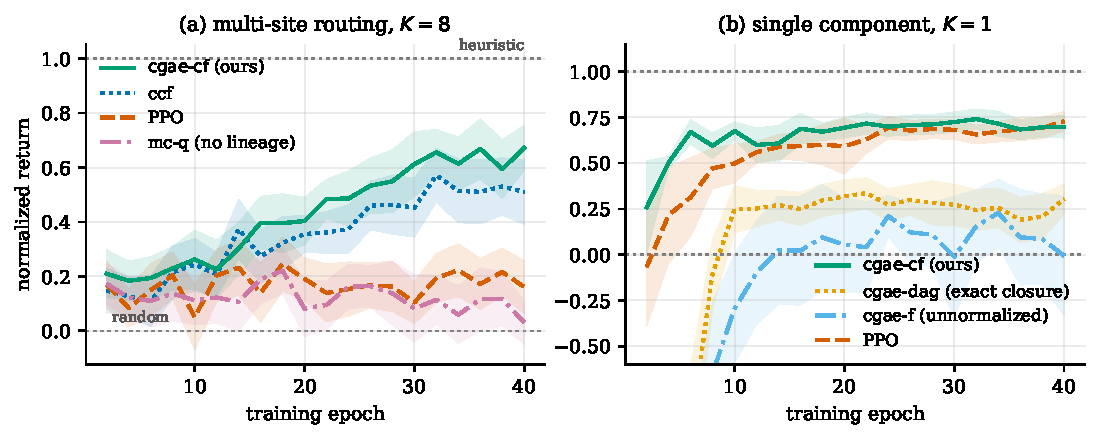
\includegraphics[width=\textwidth]{../figures/fig_curves_v3.pdf}
\caption{Learning curves, mean over $20$ common-random-number seeds with $95\%$
confidence bands; every series carries its own dash pattern so the figure reads
in greyscale. \textbf{(a)} Where the problem decomposes ($K{=}8$), causal-order
credit separates from PPO early and holds the gap; the lineage ablation
\mcq---the same return-to-go without the causal restriction---tracks PPO,
locating the gain in the decomposition rather than in the discounting.
\textbf{(b)} Where it does not ($K{=}1$), \cflow{} and PPO are
indistinguishable, which is the intended negative control. The two failing
variants separate sharply here: \cdag{} plateaus at a third of the attainable
return, and \cflowraw{} climbs, turns over, and ends near random---the
divergence Proposition~\ref{prop:s} predicts for an unbounded bootstrap
coefficient. Its early confidence band extends below the axis.}
\label{fig:curves}
\end{figure}

\begin{table}[t]
\centering
\caption{Normalized final return at the converged $40$-epoch budget,
$20$ common-random-number seeds for every cell. Parenthesised values are
standard deviations; \emph{coll.} counts collapsed seeds (normalized
$\le 0.25$) out of $20$. Dashes are cells not run. Bold marks the best arm in a
row; on the single-component environment no arm is significantly best and none
is bolded. On multi-site the causal fan-out is exactly $1$, so \cflow, \cgae{}
and \cflowraw{} are provably the same algorithm and their three columns are
bit-identical---the \cflowraw{} entry there is that shared value, not a separate
run.}
\label{tab:main}
\small
\begin{tabular}{llccccccc}
\toprule
environment & $K$ & \cflow & \cgae & \ccf & \ccap & \cflowraw & \mcq & PPO \\
\midrule
multi-site   & $8.0$ & $\mathbf{0.673}$ & $0.673$ & $0.511$ & --- & $0.673$ & $0.030$ & $0.161$ \\
             &       & \tiny(0.19) & \tiny(0.19) & \tiny(0.27) & & \tiny(0.19) & \tiny(0.18) & \tiny(0.22) \\
             & coll. & $0$ & $0$ & $3$ & --- & $0$ & $17$ & $14$ \\
$N{=}8$      & $6.3$ & $\mathbf{0.999}$ & --- & $0.977$ & --- & $0.741$ & --- & $0.804$ \\
             &       & \tiny(0.03) & & \tiny(0.06) & & \tiny(0.65) & & \tiny(0.23) \\
             & coll. & $0$ & --- & $0$ & --- & $3$ & --- & $0$ \\
$N{=}4$      & $3.3$ & $0.980$ & $\mathbf{0.995}$ & $0.974$ & $0.971$ & $0.989$ & $0.562$ & $0.715$ \\
             &       & \tiny(0.09) & \tiny(0.03) & \tiny(0.10) & \tiny(0.10) & \tiny(0.03) & \tiny(0.29) & \tiny(0.27) \\
             & coll. & $0$ & $0$ & $0$ & $0$ & $0$ & $5$ & $1$ \\
$N{=}2$      & $2.0$ & $\mathbf{0.882}$ & $0.797$ & $0.799$ & $0.761$ & $0.751$ & $0.651$ & $0.802$ \\
             &       & \tiny(0.18) & \tiny(0.30) & \tiny(0.30) & \tiny(0.43) & \tiny(0.34) & \tiny(0.39) & \tiny(0.30) \\
             & coll. & $1$ & $3$ & $3$ & $3$ & $4$ & $5$ & $3$ \\
single comp. & $1.0$ & $0.699$ & $0.643$ & $0.727$ & $0.722$ & $-0.006$ & $0.675$ & $0.729$ \\
             &       & \tiny(0.14) & \tiny(0.19) & \tiny(0.13) & \tiny(0.15) & \tiny(0.75) & \tiny(0.10) & \tiny(0.12) \\
             & coll. & $0$ & $1$ & $0$ & $0$ & $10$ & $0$ & $0$ \\
\bottomrule
\end{tabular}
\end{table}

\begin{table}[t]
\centering
\caption{Paired comparisons against \cflow{} ($20$ seeds, paired $t$-test).
The pattern is uniform: large and significant against non-causal or
unbounded-coefficient baselines, null against every bounded causal variant.}
\label{tab:paired}
\small
\begin{tabular}{llrrl}
\toprule
environment & comparator & difference & $p$ & \\
\midrule
multi-site & PPO        & $+0.512$ & $<0.0001$ & $\ast\!\ast\!\ast$ \\
multi-site & \mcq       & $+0.642$ & $<0.0001$ & $\ast\!\ast\!\ast$ \\
multi-site & \ccf       & $+0.162$ & $0.0500$  & borderline \\
$N{=}8$    & PPO        & $+0.194$ & $0.0019$  & $\ast\!\ast$ \\
$N{=}8$    & \cflowraw  & $+0.258$ & $0.0999$  & \\
$N{=}8$    & \ccf       & $+0.021$ & $0.24$    & null \\
$N{=}4$    & \mcq       & $+0.418$ & $<0.0001$ & $\ast\!\ast\!\ast$ \\
$N{=}4$    & \cfgae     & $+0.370$ & $0.0005$  & $\ast\!\ast\!\ast$ \\
$N{=}4$    & PPO        & $+0.264$ & $0.0009$  & $\ast\!\ast\!\ast$ \\
$N{=}4$    & \cgae, \ccf, \ccap, \cflowraw & $-0.015$ to $+0.009$ & $\ge 0.43$ & null \\
$N{=}2$    & \mcq       & $+0.230$ & $0.0100$  & $\ast$ \\
$N{=}2$    & all other arms & $+0.080$ to $+0.204$ & $\ge 0.052$ & null \\
single comp. & \cflowraw & $\mathbf{+0.705}$ & $\mathbf{0.0006}$ & $\ast\!\ast\!\ast$ \\
single comp. & \cdag     & $\mathbf{+0.395}$ & $\mathbf{<0.0001}$ & $\ast\!\ast\!\ast$ \\
single comp. & PPO, \cgae, \ccap, \cfgae, \ccf, \mcq & $-0.040$ to $+0.056$ & $\ge 0.27$ & null \\
\bottomrule
\end{tabular}
\end{table}

\paragraph{Against PPO the effect is large where $K$ is large.}
On multi-site, \cflow{} improves normalized return by $+0.512$ ($18$W/$1$L,
$p<0.0001$) and collapses on $0$ of $20$ seeds against PPO's $14$. At eight
copies the paired gain is $+0.194$ ($p=0.0019$), at four copies $+0.264$
($p=0.0009$), and against \cfgae{} at four copies $+0.370$ ($p=0.0005$). At two
copies the gain is $+0.080$ and not significant ($p=0.34$), and at $K{=}1$ it is
$-0.030$; the effect is therefore present at the three high-$K$ configurations
and absent at the two low-$K$ ones, which is the pattern
Proposition~\ref{prop:k} predicts and which we return to in
Section~\ref{sec:scaling}.

\paragraph{The gain is located in the causal restriction, not the discounting.}
The lineage ablation \mcq{} is the identical SMDP return-to-go with the causal
restriction removed and everything else---discounting, normalization,
optimizer---held fixed. It loses to \cflow{} on every environment where scoping
is possible, and by margins that track $K$: $+0.642$ on multi-site
($20$W/$0$L, $p<0.0001$, where \mcq{} scores $0.030$ and collapses on $17$ of
$20$ seeds), $+0.418$ at four copies ($18$W/$2$L, $p<0.0001$) and $+0.230$ at
two copies ($10$W/$4$L, $p=0.010$). On the single-component environment, where
Proposition~\ref{prop:k} says there is nothing to scope, the same ablation is
null: $+0.024$, $p=0.52$. The ablation therefore separates exactly where the
mechanism says it should and nowhere else.

\paragraph{Against other bounded causal schemes the effect is null everywhere.}
At four copies \cflow{} versus \cgae{}, \ccf{}, \ccap{} and \cflowraw{} spans
$-0.015$ to $+0.009$, every $p\ge0.43$; on the single-component environment
$-0.040$ to $+0.056$, every $p\ge0.27$; at two copies $+0.080$ to $+0.204$,
every $p\ge0.052$. (The comparison set here is the bounded causal schemes; the
non-causal ablation \mcq{} is significant at two and four copies, as reported
above.) We state this explicitly because an earlier version of this
work, run at a shorter budget with fewer seeds, reported a significant advantage
over \ccf{}; that difference was a convergence-speed artifact---\ccf{} gains
$+0.24$ at four copies under the longer budget---and it does not survive.
Multi-site is the one borderline case ($+0.162$, $p=0.0500$, $11$W/$9$L), which
we read as no reliable difference given the disagreeing rank test.

\paragraph{On the negative control the method is null, as designed.}
Against PPO on the single-component environment, \cflow{} is $-0.030$
($p=0.46$), and indeed \emph{seven} arms lie within $0.06$ of one another there.
The mechanism predicts this: $K=1.0$ and one component holds $100\%$ of reward
mass, so there is nothing to scope. A method that predicts its own failure case
is the strongest evidence we can offer for the mechanism, and the value of the
environment is that it is where the \emph{ablations} separate
(Section~\ref{sec:exp}, Table~\ref{tab:paired}).

\paragraph{The unbounded coefficient fails on the highest-$K$ environment too.}
At the shorter budget and five seeds, \cflowraw{} appeared healthy at eight
copies ($0.994\pm0.014$). At $20$ seeds it measures $0.741\pm0.654$ with $3$
collapsed seeds, against \cflow's $0.999\pm0.025$ and no collapses
($+0.258$, $p=0.0999$). Together with the single-component result
($+0.705$, $p=0.0006$), this establishes that the divergence of
Proposition~\ref{prop:s} is not a property of one environment: it appears at
both ends of the decomposability range, and it is invisible at small seed
counts because it manifests as occasional catastrophic runs rather than as a
uniformly lower mean.

\subsection{The successor normalization is necessary}

\begin{table}[t]
\centering
\caption{Single-component environment ($K{=}1$), $20$ seeds, normalized final
return, paired against \cflow. Only two rungs of the ladder are significant;
every bounded variant---PPO and the lineage ablation \mcq{} included---is
indistinguishable from every other.}
\label{tab:ablation}
\begin{tabular}{lccl}
\toprule
variant & final (SD) & collapses & paired vs \cflow \\
\midrule
\cfgae     & $0.739$ {\tiny(0.11)} & $0$ & $-0.040$ ($p=0.27$) \\
PPO        & $0.729$ {\tiny(0.12)} & $0$ & $-0.030$ ($p=0.46$) \\
\ccf       & $0.727$ {\tiny(0.13)} & $0$ & $-0.028$ ($p=0.54$) \\
\ccap      & $0.722$ {\tiny(0.15)} & $0$ & $-0.023$ ($p=0.55$) \\
\cflow     & $0.699$ {\tiny(0.14)} & $0$ & --- \\
\mcq       & $0.675$ {\tiny(0.10)} & $0$ & $+0.024$ ($p=0.52$) \\
\cgae      & $0.643$ {\tiny(0.19)} & $1$ & $+0.056$ ($p=0.36$) \\
\cdag      & $0.304$ {\tiny(0.19)} & $8$ & $\mathbf{+0.395}$ ($\mathbf{p<0.0001}$) \\
\cflowraw  & $-0.006$ {\tiny(0.75)} & $\mathbf{10}$ & $\mathbf{+0.705}$ ($\mathbf{p=0.0006}$) \\
\bottomrule
\end{tabular}
\end{table}

Two rungs of the ladder are significant and the rest are not. The
predecessor-normalized form \cflowraw{} and the exact-closure form \cdag{} both
lose decisively; the choice between flow-weighted, uniform, and sub-stochastic
predecessor handling does not matter.

\paragraph{\cflowraw{} diverges with training, exactly as Proposition~\ref{prop:s}
predicts.} The signature is visible within a single budget, without appeal to a
second one. Averaged over the same $20$ seeds, \cflowraw{} reaches a
best-checkpoint value of $0.443$ and ends at $-0.006$: a within-run drop of
$0.449$, against $0.089$--$0.136$ for every arm that learns and $0.212$ for
\cdag. It is not that \cflowraw{} fails to find a good policy---it finds one and
then destroys it. Ten of its $20$ seeds end collapsed while only two ever
collapse at their best checkpoint. One seed's greedy curve rises to $10.3$,
holds for six evaluation points, then falls to $0.15$---normalized $-1.97$, far
below random---while policy entropy stays flat at $0.18$: a confident collapse,
not an exploration failure. Extending the budget makes it worse rather than
better, which is what an error term proportional to the critic must produce: the
estimator worsens as the critic improves.

\paragraph{Reporting metric.} Tables~\ref{tab:main} and \ref{tab:ablation}
report final greedy return, as everywhere else in this paper. Because this
environment is documented as drift-prone, and because final return is the metric
most contaminated by scenario noise---which is why best-checkpoint restoration
exists in the first place---we also give the best-checkpoint reading, under
which both significant results and the whole ordering are unchanged:
\cflowraw{} $0.443$ {\tiny(0.14)} ($+0.390$ against \cflow, $20$W/$0$L,
$p<0.0001$) and \cdag{} $0.516$ {\tiny(0.15)} ($+0.316$, $19$W/$0$L,
$p<0.0001$), against \cflow's $0.833$ {\tiny(0.08)}, with every remaining arm
within $0.041$ of \cflow{} and no $p$ below $0.13$. The magnitudes shrink under
best-checkpoint precisely because checkpoint restoration is a partial guard
against the late-training divergence described above; no conclusion in this
section depends on the choice.

\subsection{Fidelity to the causal estimand does not predict performance}

\cdag{} computes the target identity of \eqref{eq:unroll} \emph{exactly}: its
measured identity ratio is $1.000$ against \cflow's $0.626$, it reproduces
textbook GAE on a chain to machine precision, and it counts a re-convergent
diamond's reward once rather than twice. It is the unbiased member of the family.
It ranks second-worst of nine. The structural reason is visible in
Table~\ref{tab:envs}: on a single-component environment the descendant closure is
most of the remaining episode ($S=0.474$, and $0.712$ on a related environment),
so the exact estimand approaches the unscoped return and exactness buys no
scoping at all.

\gapdisc{This subsection is the paper's most interesting claim and currently
rests on an association rather than an isolated mechanism. Four candidate
explanations were tested and falsified---postpone-driven action dependence, DAG
sparsity, per-state ranking fidelity against a measured counterfactual
(\emph{inverted}: \cdag{} $\rho=+0.681$ and top-1 agreement $83.3\%$ against
\cflow's $+0.435$ and $33.3\%$), and credit signal-to-noise ratio
(\emph{inverted}). The only variable separating working from failing arms is
final policy entropy ($0.27$--$0.56$ against $0.13$--$0.15$, no overlap), and
whether that is cause or symptom is untested; the decisive experiment is an
entropy-bonus intervention. All four probes were static and used a random policy,
which may simply be the wrong regime. Decide before submission whether to
present this as an open question (honest, and defensible) or to run the
intervention.}

\subsection{Scaling}
\label{sec:scaling}

The gain over PPO is present at every $K>1$ and absent at $K=1$, but it is
\emph{not} monotone in $K$:

\begin{center}
\begin{tabular}{lccc}
\toprule
environment & $K$ & gain over PPO & $p$ \\
\midrule
single component & $1.0$ & $-0.030$ & $0.46$ \\
$N{=}2$ copies   & $2.0$ & $+0.080$ & $0.34$ \\
$N{=}4$ copies   & $3.3$ & $\mathbf{+0.264}$ & $\mathbf{0.0009}$ \\
$N{=}8$ copies   & $6.3$ & $+0.194$ & $\mathbf{0.0019}$ \\
multi-site       & $8.0$ & $\mathbf{+0.512}$ & $\mathbf{<0.0001}$ \\
\bottomrule
\end{tabular}
\end{center}

We report the non-monotonicity rather than smoothing it, because its cause is
visible and is not about $K$. At $N{=}8$ every causal arm saturates near the
heuristic ($0.977$--$0.999$, standard deviations $0.03$--$0.06$) and PPO itself
reaches $0.805$, leaving under $0.20$ of headroom for any method to claim; the
gain is compressed by the ceiling, not by weaker structure. The same effect,
more mildly, explains $N{=}2$. \textbf{The defensible claim is therefore that $K$
predicts \emph{whether} component-scoped credit can help, not \emph{how much}}:
it is a screening statistic, and the magnitude additionally requires headroom.
We do not fit a trend through these five points.

\gapdisc{Also pending: whether the $N=2$ point belongs in the paper at all. At
the converged budget the spread across all seven arms there is $0.169$ and
nothing is significant, while at the shorter budget it was $0.576$ and
significant in the wrong direction. The defensible use is as the low-$K$ end of
the scaling curve, explicitly not as a method comparison.}

%===========================================================================
%===========================================================================
\section{The boundary-condition investigation}
\label{sec:boundary}
%===========================================================================


Proposition~\ref{prop:k} makes a sharp prediction: \cflow's variance reduction
scales with the number of causally independent components $K$, and collapses
to \emph{exactly} PPO when $K=1$ (a single shared resource pool links every
case into one component). This is the theorem's own honest null, not a
failure. We use a two-stage service-line environment with a single shared,
skill-heterogeneous employee pool as the decisive $K{=}1$ case. This is the
same environment called \emph{single component} in Section~\ref{sec:exp}; here
we call it the \emph{bottleneck environment} to name the mechanism under test
rather than the statistic. Its experiments predate the converged-budget re-runs
and use a $30$-epoch, $10$-seed protocol, which is why the baseline arm reads
$0.739$ here against $0.729$ in Table~\ref{tab:ablation}; see
Appendix~\ref{app:boundary}, which also gives the technical detail of all three
mechanisms. We ask: can the residual gap on
this genuinely single-component problem be closed by any other provenance- or
structure-based route? We tested three independent, well-motivated
candidates---never touching credit, only what the learner observes---and
found each provably inert or empirically neutral. Table~\ref{tab:boundary}
and Figure~\ref{fig:boundary} summarize, and Figure~\ref{fig:phidial} gives the
reward-shaping coefficient dial in full; we report all three not as a coda but
as a result, since two of the three failures follow from a proof rather than a
correlation and together they localize the bottleneck's difficulty precisely.

\paragraph{Reward shaping.} Potential-based shaping from PN topology
\citep{ng1999shaping}, SMDP-generalized, is provably policy-invariant for any
potential function---verified directly in code via an exact terminal-value
cancellation test, not merely cited. A full coefficient dial on the
bottleneck environment (same cached PPO baseline reused across all four
points) shows reach-rate cleanly monotonic in the injected-variance
direction ($8/10\to4/10\to1/10$ seeds reaching $95\%$ of the heuristic
anchor as the coefficient rises $0.2\to0.5\to1.0$), and no coefficient
produces a significant win: $0.739\pm0.10$ (baseline) vs.\ $0.766\pm0.10$
($p=.48$, coefficient $0.2$) vs.\ $0.420\pm0.10$, $0$W/$10$L (coefficient
$1.0$). The mechanism is that constant exogenous arrivals make the potential
rise as well as fall, injecting a per-step signal on the same order of
magnitude as the full episode return---unbiased in aggregate (guaranteed by
the theorem) but a substantially noisier value-regression target at a finite
budget.

\paragraph{Structural input features.} Static, conflict-graph-derived scalars
appended to each action node's own input features (does this action type
structurally compete for a token, and with how many; and, after a first null
result, the minimum topological distance to the nearest reward among an
action's required inputs) are both statistically neutral ($p=.58$ and
$p=.69$ respectively). The stronger finding is \emph{why}: every action node
already carries a one-hot action-type identity at zero hops, so the two
competing action types in the bottleneck environment are already fully
distinguishable with or without any structural feature. Any scalar computed
as a function of action type alone is therefore a deterministic function of
information a single learned weight on the one-hot could already
reconstruct---provably redundant, not merely observed to be unhelpful across
two experiments, and true of this architecture on any topology, not only the
bottleneck environment.

\paragraph{Actor architecture.} We identify and prove a previously
undocumented limitation: the actor decodes each action's logit from only that
action node's own final message-passing embedding, unlike the critic, which
has always pooled over all action/postpone node embeddings for its value
estimate. Combined with graph edges directed strictly along token flow (no
reverse edges at any real observation call site), an action's logit can
depend on state only via a forward path reaching it within the network's
depth. We prove this is a hard architectural fact, not a training-budget
limitation: on a purpose-built topology of two structurally independent
two-stage pipelines, perturbing one pipeline's downstream marking left the
other pipeline's action logit \emph{exactly, bit-for-bit unchanged} under a
randomly initialized, untrained network ($\Delta=0.000$)---reachability is a
property of the computational graph, independent of learned weights. We fix
this (concatenating the same pooled context the critic already computes onto
each action node before decoding), confirm the fix closes the gap on the
same proof topology ($\Delta=0.000\to0.528$), and re-test on the bottleneck
environment: norm.\ final $0.739\pm0.10$ (baseline) vs.\ $0.746\pm0.14$
(fixed architecture), $p=.91$---no significant effect. The proof and the
training result are not in tension: the bottleneck environment's shared
resource pool happens to recycle, giving the unfixed architecture a
marginal, accidental backdoor to the same information, so the blind spot was
never total there, and whatever fraction the fix newly exposes is not, in
practice, decision-relevant enough to move a well-tuned baseline at this
training budget.

\begin{table}[t]
\centering
\caption{The boundary-condition investigation, bottleneck environment
($K{=}1$).}
\label{tab:boundary}
\begin{tabular}{lll}
\toprule
mechanism & theoretical status & result \\
\midrule
Reward shaping & policy-invariant, any potential & neutral (0.2) to harmful (1.0), $0$W/$10$L \\
Structural input features & mechanically correct & neutral, $p=.58\to.69$; provably redundant \\
Actor global context & proven to close a real gap & neutral, $p=.91$; gap was already marginal here \\
\bottomrule
\end{tabular}
\end{table}

\begin{figure}[t]
\centering
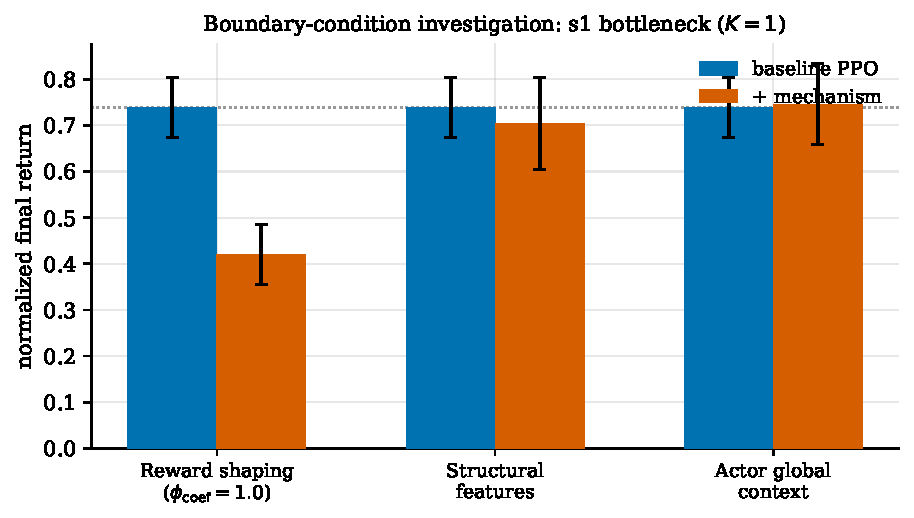
\includegraphics[width=0.78\linewidth]{../figures/fig4_boundary_summary.pdf}
\caption{Baseline PPO vs.\ each of the three boundary-condition mechanisms on
the bottleneck environment ($K{=}1$; error bars are $95\%$ CIs over seeds).
None significantly improves on the baseline; reward shaping at
$\phi_{\mathrm{coef}}{=}1.0$ is significantly worse.}
\label{fig:boundary}
\end{figure}

\begin{figure}[t]
\centering
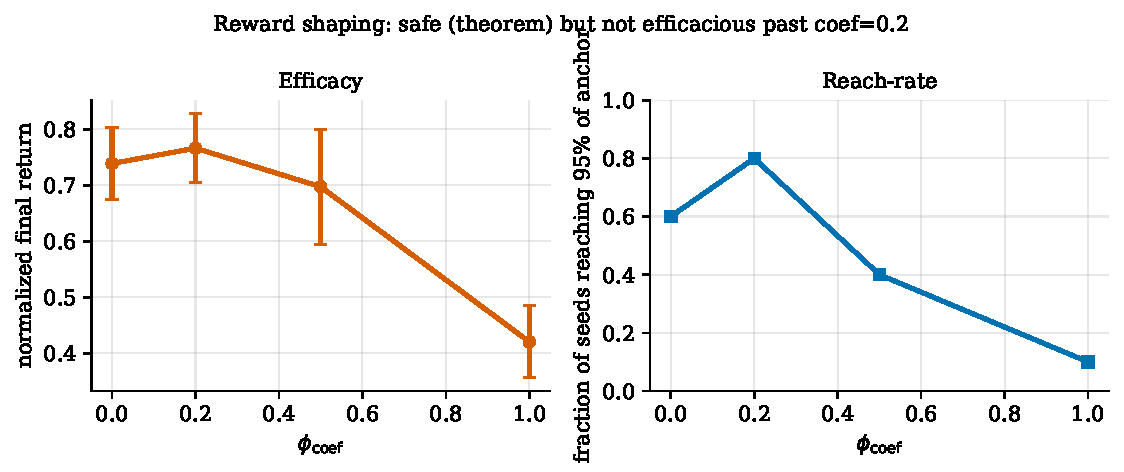
\includegraphics[width=\linewidth]{../figures/fig5_phi_dial.pdf}
\caption{The reward-shaping coefficient dial on the bottleneck environment:
efficacy (left) degrades once past $\phi_{\mathrm{coef}}=0.2$, and the
fraction of seeds reaching $95\%$ of the heuristic anchor (right) degrades
monotonically---safety (Section~\ref{sec:related}, \citealp{ng1999shaping})
and efficacy are independent properties, and this mechanism has the first
without the second at practical training budgets.}
\label{fig:phidial}
\end{figure}

None of this is a failure of experimental design: each mechanism does
exactly what it was built to do. It is evidence about where the bottleneck
environment's difficulty does \emph{not} live---not in what the learner can
observe, and not, per Proposition~\ref{prop:k}, in an avoidable credit bias
on this genuinely single-component topology. We state this as an open
problem rather than a solved one in Section~\ref{sec:discussion}.

% ======================================================================

\section{Discussion}
\label{sec:discussion}
%===========================================================================

\paragraph{A decision rule for practitioners.}
Compute $K$ from a handful of random rollouts before adopting anything. If the
problem decomposes, even partially, into weakly coupled sub-streams---parallel
lines, multiple sites, segmented resource pools---causal-order credit assignment
gives real, cheap, drop-in gains with no hand-specified structure and no forked
simulation. If $K\approx 1$, expect a null; the method is \emph{safe} there
rather than harmful, which is what Table~\ref{tab:ablation} establishes. Compute
mean fan-out as well: where it is $1$, every variant in
Table~\ref{tab:family} is the same algorithm and the implementation choice is
irrelevant.

\paragraph{What the ablation ladder teaches.}
Fidelity to a causal estimand is not the design objective; bounded error is. The
precedent is GAE itself, whose $\lambda<1$ settings are biased and universally
preferred over the unbiased $\lambda=1$ case. Our unbiased member performs worse
than three biased ones, and the one variant that fails catastrophically is the
one whose error is \emph{unbounded}.

\paragraph{Limitations.}
Five problem configurations drawn from three environment families.
\cflow{} is biased, and we verified the
action dependence of $R$ rather than assuming it away. The mechanism behind the
ladder ordering is unexplained after the six falsified hypotheses of
Appendix~\ref{app:falsified}. The bias bound of Section~\ref{sec:theory} is
stated \emph{relative} to the closure estimand $A^\star$, whose own
unbiasedness rests on Assumption~\ref{as:exo}; it is not an absolute guarantee.
That assumption is argued from A-E PN semantics rather than verified per
environment, and it is weakest exactly where a shared resource pool couples
nominally separate streams. And we
do not claim superiority over
prior component-factored schemes at converged budgets.

\gapdisc{Add a paragraph on generality across OR problem classes once a second
domain exists. The estimator requires rewards attached to discrete,
token-consuming firings, which is the real scope boundary---not the problem
domain. Admission control and network revenue management satisfy it (revenue on
acceptance); multi-item inventory does not straightforwardly, because holding
cost accrues per period rather than at a firing.}

%===========================================================================
\section{Conclusion}
%===========================================================================

An A-E PN simulation records token provenance for free, and that provenance turns
hand-specified factored credit into a derived quantity. Running generalized
advantage estimation along the provenance DAG rather than the trajectory index
yields a cheap, fork-free policy gradient that improves substantially over
discount-matched PPO wherever the problem's causal structure is even partially
decomposable, and is provably safe where it is not. The one design choice that
matters is keeping the bootstrap coefficient bounded: the natural formulation
does not, and diverges as a result.

%===========================================================================
\appendix
\section{Estimator definitions and additional remarks}
\label{app:defs}
%===========================================================================

Every arm compared in Section~\ref{sec:exp} differs from every other only in
how the per-decision target $Q[d]$ is formed. All of them are consumed
identically---the policy uses $A_d=Q[d]-V(s_d)$ and the value head regresses on
$Q[d]$---so the comparison isolates the credit rule and nothing else. Throughout,
$u_d$ is decision $d$'s clock, $t_j$ reward $j$'s firing time,
$\rho_d(t)=e^{-\beta\max(0,t-u_d)}$ the SMDP discount, $\Ascr(j)$ the decisions
on $j$'s lineage, $c(\cdot)$ the causal-component map and $\own(\cdot)$,
$\suc(\cdot)$, $\desc^{*}(\cdot)$ as in Sections~\ref{sec:method}
and~\ref{sec:estimand}.

\paragraph{Non-causal reference points.}
\begin{itemize}
\item \textbf{PPO} is the unmodified baseline: ordinary GAE along the trajectory
index with the SMDP discount, $A_t=\delta_t+\gamma\lambda A_{t+1}$.
\item \mcq{} (\emph{the lineage ablation}) is the plain Monte-Carlo SMDP
return-to-go, $Q[d]=\sum_{j:\,t_j\ge u_d}\rho_d(t_j)\,r_j$. Every decision sees
every subsequent reward whether or not it caused it. It shares the estimator
\emph{form} of the causal Monte-Carlo schemes ($\lambda=1$, no bootstrap,
wall-clock discount) and differs from them only by dropping the causal
restriction, which is exactly what makes it the ablation that prices the
lineage. It needs no token DAG.
\end{itemize}

\paragraph{Component-scoped schemes.} These restrict \emph{which} rewards a
decision sees, keeping the Monte-Carlo return-to-go.
\begin{itemize}
\item \lrq{} credits $d$ with the full discounted mass of every reward on whose
lineage it sits, $Q[d]=\sum_{j:\,d\in\Ascr(j)}\rho_d(t_j)r_j$. A reward with $k$
lineage decisions contributes its whole mass to all $k$ of them, so this is a
per-decision hindsight $Q$-sample and \emph{not} a return decomposition; it must
never be summed as a return. It is the scheme single-owner attribution
(Section~\ref{sec:method}) replaces.
\item \ccf{} builds the realized causal-component partition of
Section~\ref{sec:estimand} by union-find over each reward's lineage, then credits
$Q[d]=\sum_{j:\,c(j)=c(d),\,t_j\ge u_d}\rho_d(t_j)r_j$: its own component's
return-to-go. Because the partition is computed from the \emph{realized}
episode, component membership can itself depend on the action taken.
\item \sccf{} replaces that realized partition with a static, topology-only one
derived from the net's structure, which is action-invariant by construction. It
is reported here for completeness; it does not appear in the main tables.
\end{itemize}

\paragraph{Component-filtered GAE.}
\cfgae{} takes \ccf's partition but consumes it through PPO's own recursion
rather than as a Monte-Carlo sample: for each component it runs the ordinary
SMDP-GAE over the step-reward stream masked to that component, and each decision
reads the advantage from its own component's pass. Its $K=1$ limit is therefore
PPO \emph{exactly}---the mask is identically one and the recursion is
term-for-term PPO's---whereas every Monte-Carlo scheme above degenerates at
$K=1$ to \mcq, a different estimator that merely happens to score similarly.
That exactness is why \cfgae{} is the right comparator for "does the
\emph{partition} help, holding the estimator form fixed".

\paragraph{The causal-order family.} These run GAE's recursion along the
provenance DAG, differing only in the edge coefficient $c(d\!\to\!s)$ of
\eqref{eq:cflow}; Table~\ref{tab:family} collects the coefficients and the two
sums that matter.
\begin{itemize}
\item \cflow{} (\emph{the method}) uses $\hat w = w/R$, normalized over
successors.
\item \cgae{} uses $1/|\suc(d)|$, the equal-share special case.
\item \cflowraw{} uses the raw flow weight $w$, normalized over predecessors---
the natural formulation, and the one Proposition~\ref{prop:s} shows to be
unbounded.
\item \ccap{} uses $w/\max(R,1)$, which only ever divides, so both the
predecessor and successor sums are at most one. It prices the
share-versus-but-for choice of Remark~\ref{rem:p}.
\item \cdag{} abandons path weighting and uses set semantics: it credits each
decision with each descendant's owned reward exactly once, computing
$A^{\star}$ of \eqref{eq:star} directly. It is the unbiased member of the
family (Proposition~\ref{prop:star}).
\item \textsc{cgae-cf2} is not an ablation of any design choice but a different
DAG construction: \cflow{} with \textsc{postpone} made transparent to the
nearest-producer walk. It appears only in the discussion of that specification
wrinkle.
\end{itemize}

\paragraph{Postponement.} In every causal scheme a \textsc{postpone} decision
receives, in place of a lineage credit, the SMDP
temporal-difference advantage $e^{-\beta\tau}V(s')-V(s)$, so that every arm
gives postponement consistent support.

\begin{remark}[Why single-owner attribution rather than \lrq's lineage sample]
\lrq{} gives each reward's full mass to every decision on its lineage, so
summing its output over decisions overcounts the return by a factor that grows
with lineage depth. Single-owner attribution makes ownership a partition, which
is what turns the estimator into a return decomposition and lets the unrolled
form \eqref{eq:unroll} be read as a weighting of each reward. It also removes a
bias \lrq{} carries in the opposite direction: restricting credit to one
lineage drops the rewards that sibling lineages---the roads not taken at
$d$---would have earned, and those are causal descendants of alternative actions
at $d$, hence not mean-independent of $a_d$.
\end{remark}

\begin{remark}[Shared random streams and Assumption~\ref{as:exo}]
\label{rem:rng}
With a single global random stream, changing $a_d$ can shift the order in which
cross-component events consume random draws, so their \emph{realized} values may
differ across counterfactual actions. This affects the realized $\Delta_d$ but
not $\Ex[\Delta_d\mid\Fscr_d,a_d]$, so Assumption~\ref{as:exo}---which is a
statement about conditional means---is unaffected. The measurements in
Section~\ref{sec:exp} that fork the simulator under common random numbers
exploit exactly this distinction.
\end{remark}

All proofs are given inline where the results are stated:
Proposition~\ref{prop:star} and Proposition~\ref{prop:k} in
Section~\ref{sec:estimand}, Lemma~\ref{lem:visit} and
Proposition~\ref{prop:bias} in Section~\ref{sec:bias}, and
Proposition~\ref{prop:rel} in Section~\ref{sec:relative}. They are short enough
that separating them from the statements would cost more than it saves.

%===========================================================================
\section{Environments}
\label{app:envs}
%===========================================================================

All three environment families are Action-Evolution Petri Nets built with the
same library and solved by the same agent; they differ in topology, not in
machinery. Each grants reward $1$ per completed task, so return is throughput
over the horizon. Table~\ref{tab:envspec} collects the parameters.

\paragraph{Multi-site skills-based routing (the realistic environment).}
A firm runs four service sites. Each site has its own stochastic arrival stream
of tasks of two types and its own heterogeneous pool of dedicated specialists:
one skilled for each type, fast on their matched type (service delay $1$) and
slow otherwise (delay $3$). A specialist serves a task at its own site and
returns to that site's pool. The decision is which queued task each free worker
takes. Because every worker cycles within its own site, each worker's token
lineage links only decisions that used it, and the episode decomposes into eight
causal components---which is why this environment measures $K=8.0$ and a causal
fan-out of exactly $1$.

The environment also carries a coupling knob we do not exercise in the main
results but which motivates the design: a pool of \emph{flexible} generalists,
usable at any site (delay $2$, type-independent). A flexible worker that serves
site $i$, returns to the shared pool and then serves site $j$ links those sites'
decisions into one component. The local/flexible capacity split therefore traces
the whole independence spectrum---all-dedicated gives $n_{\mathrm{sites}}$
components, all-pooled gives one---instantiating the classical
OR question of resource pooling and flexibility as a single dial over $K$. The
reported configuration is the all-dedicated end.

\paragraph{The $N$-copies scaling benchmark.}
$N$ fully independent single-stage assignment problems in one net, served by one
shared policy, with reward summed over copies. Each copy has its own arrival
stream, queue, busy place and dedicated employee; no place is shared. A copy's
tasks are either \emph{matched} to its employee (service $1+U\{0,1\}$) or
\emph{crossed} (service $3+U\{0,1\}$), so serving matched work first maximizes
throughput. The copies are causally independent by construction, so $K\le N$
with equality whenever every copy emits a reward within the horizon
(Definition~\ref{def:k}). This is the one environment where the independence
structure is a controlled parameter rather than a measured property, which is
what makes it the scaling benchmark; it is deliberately synthetic.

\paragraph{The single-component environment (negative control).}
A two-stage service line: cases arrive stochastically, are served at stage one,
then queue for stage two, and reward is emitted on completing stage two. Both
stages draw from \emph{one shared pool of three heterogeneous employees}---two
specialists, fast on their matched type (delay $1$) and slower otherwise
($2$), plus a generalist (delay $3$)---and every employee returns to that same
pool after each service. The shared pool links every case's lineage into a
single causal component, giving $K=1.0$ with one component holding $100\%$ of
reward mass. It is the mechanism's own predicted null, and it is also the
environment of the boundary-condition investigation of
Section~\ref{sec:boundary}, where it is called the \emph{bottleneck
environment} because the shared pool is the binding constraint.

\begin{table}[t]
\centering
\caption{Environment parameters. Horizon is in simulated time units; the
heuristic is the anchor for the normalization
$(\text{score}-\text{random})/(\text{heuristic}-\text{random})$ and is a strong
myopic rule, not a proven optimum, so normalized values above $1$ are
attainable.}
\label{tab:envspec}
\small
\begin{tabular}{llccc}
\toprule
environment & structure & horizon & random & heuristic \\
\midrule
multi-site routing & $4$ sites $\times$ $2$ dedicated specialists & $20$ & $62.90$ & $80.25$ \\
$N$-copies, $N=2$  & $2$ independent copies, $1$ employee each & $20$ & $15.87$ & $22.60$ \\
$N$-copies, $N=4$  & $4$ independent copies, $1$ employee each & $20$ & $31.13$ & $44.60$ \\
$N$-copies, $N=8$  & $8$ independent copies, $1$ employee each & $20$ & $63.20$ & $89.53$ \\
single component   & $2$ stages, $1$ shared pool of $3$ & $20$ & $9.85$ & $14.78$ \\
\bottomrule
\end{tabular}
\end{table}

\paragraph{Heuristics.} All three anchors are simple priority rules and none
ever postpones. On multi-site, a specialist takes its own matched type first;
failing that a flexible worker is used; failing that any specialist takes
crossed work. On $N$-copies, a binding serving a matched (fast) task is
preferred, otherwise any enabled binding is taken. On the single-component
environment the rule prioritises by stage---work in progress at stage two
before new work at stage one---and within a stage prefers a type-matched
employee. Random baselines sample uniformly from the enabled bindings. Both
anchors are evaluated on the canonical no-postpone variant of each net, so the
normalization scale is a property of the environment rather than of the action
space the learner sees.

%===========================================================================
\section{Training setup and reproducibility}
\label{app:repro}
%===========================================================================

\paragraph{Architecture.} Policy and value networks are separate heterogeneous
graph networks over the assignment-graph representation, each a stack of three
Heterogeneous Graph Transformer convolutions \citep{hu2020hgt} with hidden width
$128$ and two attention heads, with residual connections and dropout. Places and
transitions are distinct node types. The critic pools over node embeddings to
produce a scalar; the actor decodes one logit per enabled action binding from
that binding's node embedding---the asymmetry Section~\ref{sec:boundary}
analyses. Input widths are inferred lazily from the first observation, so the
same code runs unchanged across environments with different attribute sets.

\paragraph{Optimization.} All arms share the hyperparameters of
Table~\ref{tab:hyper}; no per-arm tuning was performed, and the causal schemes
inherit the baseline's settings unchanged. This is deliberate---any tuning
advantage would confound the credit comparison---but it also means the reported
numbers are not the best attainable for any arm.

\begin{table}[t]
\centering
\caption{Hyperparameters, identical for every arm and every environment.}
\label{tab:hyper}
\small
\begin{tabular}{ll}
\toprule
parameter & value \\
\midrule
algorithm & PPO with clipped surrogate objective \\
epochs & $40$ (converged budget; $15$ and $30$ retained as ablations) \\
episodes per epoch & $20$ \\
minibatch size & $32$ \\
policy / value learning rate & $3\times10^{-4}$ / $3\times10^{-4}$ \\
policy / value update passes & $3$ / $4$ per epoch \\
clip parameter $\varepsilon$ & $0.2$ \\
entropy bonus & $0.01$ \\
KL early-stopping limit & $0.15$ (mean per-state $\mathrm{KL}(\pi_{\mathrm{old}}\Vert\pi)$) \\
discount $\gamma$ / GAE $\lambda$ & $0.99$ / $0.95$ \\
SMDP discount rate $\beta$ & $0.5$ \\
postponement & enabled \\
\bottomrule
\end{tabular}
\end{table}

\paragraph{Evaluation protocol.} Every second epoch the greedy (argmax) policy
is evaluated on $20$ episodes; the reported \emph{final} value is the last such
point and \emph{best} the maximum over them. All evaluation uses common random
numbers: with the evaluation seed fixed, evaluation episode $i$ always runs
scenario $\mathrm{seed}+i$, so every method, seed and epoch is scored on one
fixed scenario set and arms differ only by policy. This matters more than it
may appear: without it, the measured noise floor on the single-component
environment is $\pm0.231$ standard deviations per evaluation point and
$\pm0.327$ on a paired difference, and drift is inflated by roughly $0.40$ even
for a policy that is not changing. Baselines average $40$ episodes. Seeds
$0$--$19$ are used for every cell, and comparisons are paired seed-by-seed;
we report paired $t$-tests and Wilcoxon signed-rank tests, and where they
disagree we say so.

\paragraph{Determinism.} A single entry point seeds Python's \texttt{random},
NumPy and PyTorch, and is applied to environment construction, network
initialization, rollout collection and evaluation, so a cell is reproducible
from its (environment, method, seed) triple. Paired arms share their network
initialization. Each cell is written to its own result file and runs are
resumable: re-running a sweep trains only the missing cells, which is how the
arm coverage in Table~\ref{tab:main} was filled incrementally.

\paragraph{Cost.} Credit computation is a single backward pass over the
decisions of one episode, $O(|E|)$ in the provenance DAG, measured at
approximately one millisecond per episode. Against a training cell at four
copies this is under $8\%$ of wall-clock time (PPO $7.44$ minutes against
$8.05$); the graph network dominates, and profiling attributes roughly $83\%$
of a cell to the optimizer's repeated forward and backward passes over the
collected graphs. No arm requires forked simulation.

\section{Falsified mechanisms}
\label{app:falsified}

Section~\ref{sec:exp} reports that fidelity to the causal estimand does not
predict learning performance, and offers only a partial structural account of
why. That claim would be easy to dress up with a plausible mechanism. We
instead record every mechanism we tested and rejected, with the measurement
that rejected it, so a reader can judge how much of the ordering is explained
and how much is not. All six were pre-registered in the sense that the
prediction was written into the diagnostic script before it was run.

\subsection{Summary}

\begin{table}[h]
\centering
\caption{Candidate mechanisms for the ablation ordering, and the measurements
that falsified them. ``Inverted'' means the measured quantity ordered the
variants \emph{opposite} to performance.}
\label{tab:falsified}
\small
\begin{tabular}{p{4.1cm}p{5.4cm}l}
\toprule
hypothesis & measurement & outcome \\
\midrule
Postpone is the dominant source of the action-dependence of $R$ &
making postpone transparent leaves $R$ identical across actions on $50.0\%$ of
fork points, down from $68.8\%$; spread on the single-component environment
rises $0.580\to0.947$ &
\textbf{worse} \\[2pt]
Credit decays along chains as $\prod w$, so \cflowraw{} propagates less &
backward propagation mass at causal depth $5$: $0.89$ (\cflowraw) vs $0.95$
(\cflow) &
too small \\[2pt]
Larger credit magnitude gives a larger effective step &
$\mathrm{mean}|Q|$ at two copies: $2.23$ vs $2.22$; $\mathrm{SD}$ $1.10$ vs
$1.12$ &
identical \\[2pt]
Per-state ranking fidelity against a measured counterfactual &
Spearman $\rho$ / top-$1$ agreement with common-random-number counterfactual
return: \cdag{} $+0.681$ / $83.3\%$, \cflow{} $+0.435$ / $33.3\%$ &
\textbf{inverted} \\[2pt]
Credit signal-to-noise ratio (bias--variance) &
between-action signal over within-action noise: \cdag{} $0.959$ (highest),
\cflow{} $0.895$; full range $0.80$--$0.96$ &
\textbf{inverted} \\[2pt]
\cdag's arbitrary $\lambda^{k_{\min}}$ depth weighting &
replacing it with the depth-conditioned weight $\Ex[\lambda^{L}\mid\text{visit}]$
moves correlation with \cflow{} from $0.740$ to $0.748$ &
$\Delta=0.008$ \\
\bottomrule
\end{tabular}
\end{table}

\subsection{Detail}

\paragraph{Postpone transparency.}
Under token-flow postponement a \textsc{postpone} firing re-emits the entire
marking, so it terminates the nearest-producer walk without having caused the
flow, and it carries $2.25$--$2.66\times$ the row sum of production actions. We
therefore expected removing it to make $R$ closer to action-measurable. It does
the opposite. Transparency \emph{redirects} postpone's edges to the true
producers---$0$ production-to-production edges lost, $50$ gained at four copies
and $97$ on the single-component environment---and the recovered edges are
precisely the action-dependent ones. Postpone had been making $R$ look invariant
by destroying information. The resulting variant is also the worst arm we
measured ($0.106$ normalized), so the more causally faithful graph is the worse
learner---a second instance of the pattern in Section~\ref{sec:exp}.

\paragraph{Chain decay and credit magnitude.}
Both were attempts to explain a large performance gap by a mechanical property
of the credit vector, and both fail on magnitude grounds: the measured
differences are one to five percent where the performance difference to be
explained was $0.44$ in normalized return.

\paragraph{Ranking fidelity.}
This is the sharpest negative result, because it tests the estimator against
ground truth rather than against another estimator. At a decision state we fork
the simulator once per action under common random numbers and record the
realized discounted return-to-go; differences across branches are then the
causal effect of the action with the exogenous component cancelled. A credit
scheme should rank actions the way that quantity does. On the single-component
environment \cdag{} ranks them \emph{better} than \cflow{} on both measures
while learning far worse. Ranking fidelity at a fixed state therefore does not
determine learning outcome. Caveats: $12$ usable fork points, and the
continuation policy is random, so this measures counterfactual value under
random continuation rather than under the converged policy.

\paragraph{Signal-to-noise.}
We forked each production action under $M$ shared exogenous seeds and formed the
ratio of between-action to within-action credit dispersion---an $F$-ratio for
the quantity a policy gradient integrates. The prediction was that \cdag{},
whose closure sum approaches the unscoped return on a single-component problem,
would show the lowest ratio. It shows the highest. The mechanism was half right
and immaterial: \cdag{} does carry about twice the noise ($0.459$ vs $0.272$),
but it also carries about twice the signal ($0.420$ vs $0.237$), and the
scaling cancels.

\paragraph{The depth-weighting choice.}
\cdag{} weights a descendant's owned reward by $\lambda^{k}$ at minimum causal
depth $k$, which is discretionary: a re-convergent descendant reachable at
depths $2$ and $7$ receives $\lambda^{2}$. We built the principled alternative,
weighting by $\Ex[\lambda^{L}\mid\text{the walk visits } j]$, which coincides
with the closure estimand at $\lambda=1$ and inherits \cflow's depth
distribution conditioned on arrival. It changes almost nothing. The reason is
structural and is worth stating as a positive by-product: since
\[
  c^{\cflow}_d(j)\;=\;\underbrace{\Pr[\text{visit } j]}_{\text{the fan-out gap}}
  \cdot\underbrace{\Ex\bigl[\lambda^{L}\mid\text{visit } j\bigr]}_{\text{depth weighting}},
\]
the two factors are separable, and the closure variants differ from \cflow{}
only by discarding the first. The behavioural difference is the gap itself, not
any detail of how depth is discounted within the closure.

\subsection{A budget artifact, recorded for the same reason}

At the $15$-epoch budget with $20$ seeds, \cflow{} measured $0.401$ against
\cflowraw's $0.837$ at two copies ($4$W/$14$L, $p=0.0043$)---an apparently
significant deficiency in the method we ship. It is an artifact of
non-convergence. At $40$ epochs the comparison is $+0.102$ ($p=0.51$), sign
reversed. Three measurements identify the cause: a $\lambda$ sweep recovers most
of the deficit ($0.401\to0.579\to0.639$ as $\lambda$ falls
$0.95\to0.85\to0.70$ toward \cflowraw's effective $0.95\times0.896\approx0.851$),
so it is a convergence-\emph{speed} effect; the credit vectors differ by about
one percent; and the outcomes are bimodal with nothing in between. We report
this because it is the clearest evidence in this work that a significant result
at a short budget can be entirely spurious, and it is why
Section~\ref{sec:exp} reports the converged budget throughout.

\subsection{The one surviving correlate}

Across all arms and environments the single variable that separates working from
failing configurations without overlap is \emph{final policy entropy}:
$0.27$--$0.56$ for the four arms that learn, $0.13$--$0.15$ for the three that
fail. Whether this is cause or symptom is untested---a policy in a poor local
optimum will show low entropy regardless of how it arrived---and the decisive
experiment, an entropy-bonus intervention on the failing arms, has not been run.
We state the correlation and its status rather than promoting it to a mechanism.

\subsection{Methodological note}

All six diagnostics share a design feature that may explain their uniform
failure: each measures a \emph{static} property of the estimator under a
\emph{random} policy with random continuations. Training involves a learned
policy that becomes progressively deterministic, and the failures we are trying
to explain unfold over tens of epochs. It is entirely possible that no static,
random-policy property of a credit estimator predicts its training outcome. If
so, that is itself a finding about how credit-assignment methods should be
evaluated, and it argues for interventional rather than observational
diagnostics---consistent with the boundary-condition results of
Section~\ref{sec:boundary}, where only active-intervention mechanisms ever moved
the single-component floor.

%===========================================================================
\section{Boundary-condition investigation: technical detail}
\label{app:boundary}
%===========================================================================

\paragraph{Protocol, and why it differs.} The three experiments of
Section~\ref{sec:boundary} predate the converged-budget re-runs and use the
stochastic suite's standard budget: the single-component environment at $30$
epochs $\times$ $20$ episodes, $10$ seeds, paired seed-by-seed against a
\texttt{ppo\_clip} baseline, reporting normalized final return. That baseline
therefore reads $0.739\pm0.10$ here against $0.729\pm0.12$ in
Table~\ref{tab:ablation}, which is the same arm at $40$ epochs and $20$ seeds;
the difference is budget and seed count, not environment. We did not re-run them
at the longer budget because all three outcomes are nulls or negatives, and a
longer budget cannot convert a null into the positive result that would change
the section's conclusion. The environment is the one described in
Appendix~\ref{app:envs}; Section~\ref{sec:boundary} calls it the
\emph{bottleneck environment} to name the mechanism under test rather than the
statistic $K$.

\paragraph{Potential-based shaping.} The shaping term is the SMDP
generalization $F(s,a,s')=e^{-\beta\tau}\Phi(s')-\Phi(s)$, added to every step's
reward, with the potential read off the net's topology:
$\Phi(s)=\sum_p \mathrm{decay}^{\mathrm{hop}(p)}\cdot\min(|p|,\mathrm{cap})$,
a distance-decayed structural backlog in which each place's token count is
weighted by its hop-distance to the nearest reward-emitting transition and
optionally capped. Policy invariance \citep{ng1999shaping} was verified in code
by an exact terminal-value cancellation test rather than merely cited. The
coefficient dial reuses one cached baseline across all four points, so the
comparison is paired by construction.

The failure mechanism is worth stating because it is not a property of the
potential's shape. This environment has constant exogenous arrivals---one case
per time unit---so the backlog potential rises as often as it falls, and the
per-step shaping signal is of the same order of magnitude as the entire episode
return. Aggregated over an episode the term telescopes to a constant, exactly as
the theorem promises, but at any finite budget it is a substantially noisier
value-regression target. Safety and efficacy are independent properties, and
this mechanism has the first without the second.

\paragraph{Structural input features.} Two feature sets were appended to each
action node's own inputs: first, whether an action type structurally competes
for a token and with how many rivals, derived from the conflict graph; then,
after that returned a null, the minimum topological hop-distance from an
action's required inputs to the nearest reward-emitting transition. The second
does discriminate between the environment's two action types ($0.656$ against
$0.810$), so the null is not a degenerate-feature artifact.

The redundancy argument is the stronger result and does not depend on either
feature's design. Every action node already carries a one-hot action-type
identity at zero hops. Any scalar that is a function of action type alone is
therefore a deterministic function of information a single learned weight on
that one-hot could reconstruct, so it cannot add representational capacity. This
holds for this architecture on any topology, which is why we report it as a
proof rather than as two failed experiments. A structural feature can only help
if it varies \emph{within} an action type---across markings---which
conflict-degree on a two-node conflict pair provably does not.

\paragraph{Actor architecture.} The blind spot is a property of the
computational graph, not of training. The actor decodes each action's logit from
that action node's own final message-passing embedding; the graph's edges run
strictly along token flow, with no reverse edges at any real observation call
site; so an action's logit can depend on state only through a forward path
reaching it within the network's depth. The demonstration uses a purpose-built
topology of two structurally independent two-stage pipelines: perturbing one
pipeline's downstream marking leaves the other pipeline's action logit
bit-for-bit unchanged ($\Delta=0.000$) under a randomly initialized, untrained
network. Reachability does not depend on learned weights, so no training budget
can close it.

The fix concatenates onto each action node, before decoding, the same pooled
context the critic already computes---an intervention on the actor alone,
leaving the critic and the credit path untouched. On the proof topology it
closes the gap exactly ($\Delta=0.000\to0.528$). On the single-component
environment it is neutral ($0.746\pm0.14$ against $0.739\pm0.10$, $p=.91$), and
the two results are not in tension: that environment's shared resource pool
recycles workers, which gives the unfixed architecture a marginal, accidental
path to the same information within three hops. The blind spot was never total
there, and whatever fraction the fix newly exposes is not decision-relevant
enough to move a well-tuned baseline at this budget. The architectural finding
stands on the proof; the training result bounds its practical value on this
environment only.

\bibliographystyle{elsarticle-harv}
\bibliography{refs}

\end{document}
